%\documentclass{article}
\documentclass[10pt,a4paper]{book}
\usepackage[a4paper,bindingoffset=0.2in,%
            left=1in,right=1in,top=1in,bottom=1in,%
            footskip=.25in]{geometry}

\usepackage[utf8]{inputenc}

\title{Book of Solutions}
\author{C Thierfelder}
\date{May 2020}


%MATH
\usepackage{amsmath}
\usepackage{amsfonts}
\usepackage{amsthm}
\usepackage{units}
\usepackage{mathrsfs}

\usepackage{hyperref}


\newtheorem{remark}{Remark}[section]
\theoremstyle{definition}
\newtheorem{definition}{Definition}[section]
\newtheorem{theorem}{Theorem}[section]

\DeclareMathOperator{\Aut}{Aut}
\DeclareMathOperator{\GL}{GL}

%PAGELAYOUT
\usepackage{a4wide}

%GRAPHICS
\usepackage{graphicx}
\usepackage[dvipsnames]{xcolor}
\usepackage{tikz}
\usepackage[outline]{contour} % glow around text

\usetikzlibrary{shapes}
\usetikzlibrary{plotmarks}
\usetikzlibrary{decorations.markings}

\usepackage{pgfplots}
\usepgfplotslibrary{polar}

%HYPERLINKS
\usepackage{hyperref}
\hypersetup{
    colorlinks=true,
    linkcolor=blue,
    filecolor=magenta,      
    urlcolor=cyan,
}

\usepackage[shortlabels]{enumitem}

\usepackage{etoolbox}
\providetoggle{includeCoverPic}
\settoggle{includeCoverPic}{true}
%\settoggle{includeCoverPic}{false}

\usepackage{subfiles}
\begin{document}

\maketitle

\chapter{Introduction}
There is a theory which states that if ever anyone discovers exactly what the Universe is for and why it is here, it will instantly disappear and be replaced by something even more bizarre and inexplicable.
There is another theory which states that this has already happened.

\iftoggle{includeCoverPic}{
\begin{center}
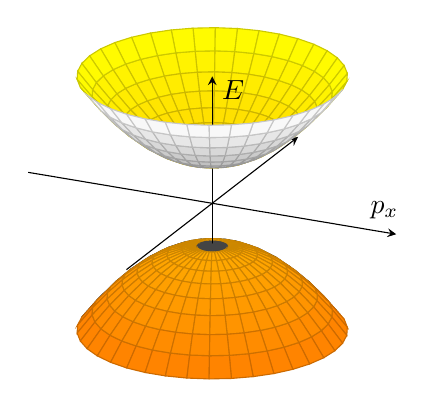
\begin{tikzpicture}
\begin{axis}[
  axis lines=none,
  %xlabel={$p_x$}, ylabel={$p_y$}, zlabel={$E$},
  domain=0:1,
  y domain=0:pi,
  xmin=-1.5, xmax=1.5,
  ymin=-1.5, ymax=1.5, zmin=-1.5, zmax=1.5,
  mesh/interior colormap={blueblack}{color=(orange) color=(yellow)},
  colormap/blackwhite, 
  samples=10,
  samples y=20,
  z buffer=sort,
  ticks=none,
 ]
  \addplot3[surf]  ({x*cos(deg(y))},{x*sin(deg(y))},{+x^2+0.5});
  \addplot3[surf]  ({x*cos(deg(y))},{x*sin(deg(y))},{-x^2-0.5});
\end{axis}

\begin{axis}[
  axis lines=center,
  xlabel={$p_x$}, zlabel={$E$},
  domain=0:1,
  y domain=pi:2*pi,
  xmin=-1.5, xmax=1.5,
  ymin=-1.5, ymax=1.5, zmin=-1.5, zmax=1.5,
  mesh/interior colormap={blueblack}{color=(orange) color=(yellow)},
  colormap/blackwhite, 
  samples=10,
  samples y=20,
  z buffer=sort,
  ticks=none,
 ]
  \addplot3[surf] ({x*cos(deg(y))},{x*sin(deg(y))},{+x^2+0.5});
  \addplot3[surf] ({x*cos(deg(y))},{x*sin(deg(y))},{-x^2-0.5});
\end{axis}

\end{tikzpicture}
\end{center}
}


\newpage
\tableofcontents

%SECTION_NUMBERING
\setcounter{secnumdepth}{2}


\newpage
\chapter{Useful formulas}
\subfile{sections/00usefulFormulas}

\newpage
\chapter{Primers}
\subfile{sections/01Primers}

\chapter{Groups}
\subfile{sections/02Groups}

\newpage
\chapter{Mathematical}
\subfile{sections/03Mathematical}

\chapter{Classical Mechanics}
\subfile{sections/18CM}

\chapter{Electrodynamics}
\subfile{sections/14ED}

\chapter{Quantum Mechanics}
\subfile{sections/13QM}

\chapter{Thermodynamics and Statistical Physics}
\subfile{sections/15TDST}

\chapter{Many-body physics}
\subfile{sections/04ManyBody}

\chapter{Quantum Field Theory}
\subfile{sections/05QFT}

\chapter{Particle Physics}
\subfile{sections/07ParticlePhysics}

\chapter{Nuclear Physics}
\subfile{sections/06NuclearPhysics}

\chapter{Astrophysics}
\subfile{sections/11Astrophysics}

\chapter{General Relativity}
\subfile{sections/08GR}

\chapter{Cosmology}
\subfile{sections/12Cosmology}

\chapter{Quantum Gravity}
\subfile{sections/09QuantumGravity}

\chapter{String Theory}
\subfile{sections/10StringTheory}

\chapter{Landau Lifschitz}
\subfile{sections/16Landau}

\chapter{General Physics}
\subfile{sections/17GenPhys}


\newpage
\chapter{Simulations of Cosmic Structure Formation - MAUCA 2018}
\subsection{Exercise 2}
\begin{enumerate}
\item Summary of Friedmann equations
We start with the total energy density
\begin{align}
\rho=\frac{3H_0^2}{8\pi G}\left[
\Omega_\Lambda+
\Omega_m\left(\frac{a_0}{a}\right)^3+
\Omega_r\left(\frac{a_0}{a}\right)^4\right]
\end{align}
Using the Friedman equation we get
\begin{align}
\dot{a}^2+K
&=\frac{8\pi G\rho a^2}{3}\\
\dot{a}^2-\Omega_Ka_0^2H_0^2&=a^2H_0^2\left[
\Omega_\Lambda+
\Omega_m\left(\frac{a_0}{a}\right)^3+
\Omega_r\left(\frac{a_0}{a}\right)^4\right]\\
\dot{a}^2&=a^2H_0^2\left[
\Omega_\Lambda+
\Omega_m\left(\frac{a_0}{a}\right)^3+
\Omega_r\left(\frac{a_0}{a}\right)^4+
\Omega_K\left(\frac{a_0}{a}\right)^2\right]
\end{align}
where we used $\Omega_K=-K/(a_0H_0)^2$. With $a(t_0)=a_0$ and $H_0\equiv\frac{\dot{a}(t_0)}{a(t_0)}$ we find a constraint on the $\Omega$ parameters
\begin{align}
\Omega_\Lambda+\Omega_m+\Omega_r+\Omega_K=1
\end{align}
Then with $x=a/a_0$
\begin{align}
\dot{x}^2&=x^2H_0^2\left[
\Omega_\Lambda+
\Omega_m x^{-3}+
\Omega_r x^{-4}+
\Omega_K x^{-2}\right]\\
\frac{dx}{dt}&=H_0\sqrt{
\Omega_\Lambda x^2+
\Omega_m x^{-1}+
\Omega_r x^{-2}+
\Omega_K}\\
H_0dt&=
\frac{dx}{\sqrt{
\Omega_\Lambda x^2+
\Omega_m x^{-1}+
\Omega_r x^{-2}+
\Omega_K}}
\end{align}
\item Solutions
\begin{align}
\dot{x}&=H_0\sqrt{
\Omega_\Lambda x^2+
\Omega_m x^{-1}+
\Omega_r x^{-2}+
\Omega_K}
\end{align}
\begin{itemize}
\item $k=0, \Omega_\Lambda=1,\Omega_m=\Omega_r=0$
\begin{align}
\dot{x}=H_0x\quad\rightarrow\quad x=e^{H_0t}
\end{align}

\item $k=0, \Omega_m=1,\Omega_\Lambda=\Omega_r=0$
\begin{align}
\dot{x}=H_0x^{-1/2}\quad\rightarrow\quad x=\left(1+\frac{3}{2}H_0t\right)^{2/3}
\end{align}

\item $k=0, \Omega_r=1,\Omega_\Lambda=\Omega_m=0$
\begin{align}
\dot{x}=H_0x^{-1}\quad\rightarrow\quad x=1+H_0t
\end{align}


\end{itemize}
\end{enumerate}
\newpage
\chapter{Doodling I}
\section{Basic Principles}
Relativistic QFT unifies quantum mechanics ($\hbar$) and special relativity ($c$). We will put $\hbar=1=c$.
\begin{itemize}
\item Relativistic Invariance

Coordinates and how they transform
\begin{align}
x^\mu&=(ct,\vec{x}), \qquad \partial_\mu=\frac{\partial}{\partial x^\mu}\\
x^\mu&\rightarrow x'^{\mu}=a^\mu+\Lambda^\mu_{\;\nu}x^\nu
\end{align}
All transformations ($a$,$\Lambda$) - translations and Lorentz transformations - build the Poincare group $\mathcal{P}$.
\begin{align}
x^\mu x_\mu=x^\mu x^\nu\eta_{\mu\nu}, \qquad \eta=\text{diag}(1,-1,-1,-1)
\end{align}
Invariance requirement
\begin{align}
x'^2\overset{!}{=}x^2\quad\Rightarrow\quad \Lambda_\mu^{\;\rho}\Lambda_\nu^{\;\sigma}\eta_{\rho\sigma}\overset{!}{=}\eta_{\mu\nu}
\end{align}
\end{itemize}

\section{Representation Theory of the Poincare group}
\begin{itemize}
\item Relevant because: elementary particles  = unitary, irreducible representation of the Poincare group $\mathcal{P}$.

\item But there are no finite dimensional unitary representations of non-compact groups $\rightarrow$ $\infty$-dimensional representation (need Hilbert space).

\item So each transformation
\begin{align}
x^\mu&\rightarrow x'^{\mu}=a^\mu+\Lambda^\mu_{\;\nu}x^\nu
\end{align}
will be represented by some unitary operator $U(a,\Lambda)$ ( with $U^\dagger=U^{-1}$) acting on some infinitely dimensional Hilbert space.

\item Let's look at pure translations first
\begin{align}
U(a,1)\equiv U(a)=e^{ia^\mu P_\mu}
\end{align}
with the generators (the momentum operator) of the translations $P_\mu=(H,\vec{P})$ with needs to be hermitian $P_\mu=P^\dagger_\mu$.
\item For the pure Lorentz transformations we get
\begin{align}
U(0,\Lambda)\equiv U(\Lambda)=e^{\frac{i}{2}\omega_{\mu\nu} M^{\mu\nu}}
\end{align}
with the generators of the Lorenz transformations $M^{\mu\nu}$ which need to obey $M_{\mu\nu}=M^\dagger_{\mu\nu}$. They can be identified by $M^{12}\equiv J^3$, $M^{23}\equiv J^1$ and $M^{31}\equiv J^2$ with the angular momentum operator $\vec{J}$ (generating rotations) and generators of the Lorentz boosts $M_{0i}$.

\item Lets derive the commutation operator of the generators. Translations commute therefore
\begin{align}
U(a_1)U(a_2)=U(a_1+a_2)=U(a_2)U(a_1)\quad\Rightarrow\quad
\boxed{[P_\mu,P_\nu]=0}
\end{align}
In general
\begin{align}
(a_1,\Lambda_1)\circ(a_2,\Lambda_2)=(a_1+\Lambda_1a_2,\Lambda_1\Lambda_2)
\end{align}
Then the representation need to obey
\begin{align}
U(a_1,\Lambda_1)U(a_2,\Lambda_2)=U(a_1+\Lambda_1a_2,\Lambda_1\Lambda_2)
\end{align}
which for $\Lambda_1=\Lambda$, $\Lambda_2=\Lambda^{-1}$, $a_2=a$ and $a_1=0$
\begin{align}
U(0,\Lambda)U(a,\Lambda^{-1})&=U(\Lambda a,1)\\
\rightarrow U(\Lambda)U(a)U(\Lambda^{-1})&=U(\Lambda a)
\end{align}
In lowest order this results in
\begin{align}
\boxed{[M_{\rho\sigma},P_\mu]=i\eta_{\mu\rho}P_\sigma-i\eta_{\mu\sigma}P_\rho }
\end{align}
\begin{align}
\boxed{[M^{\mu\nu},M^{\rho\sigma}]=i\eta^{\mu\rho}M^{\nu\sigma}+i\eta^{\nu\sigma}M^{\mu\rho}-i\eta^{\mu\nu}M^{\rho\sigma}-i\eta^{\rho\sigma}M^{\mu\nu}}
\end{align}
From this we can recover $[J^i,J^k]=i\varepsilon^{ijk}J^k$ , $[H,\vec{P}]=0$, $[H,\vec{J}]=0$ (angular momentum conservation) and $[H,M_{0i}]\neq0$ (not conserved).
\end{itemize}

How to classify irreps:
\begin{itemize}
\item recall QM: SO(3) use the Casimir operator $\vec{J}^2$ (operator that commutes with all generators, $J_1, J_2, J_3$) 
\begin{itemize}
\item use it to label all irreducible representations
\item use $J_3$ to label the states within the representation
\end{itemize}  
\item Casimir operators for $\mathcal{P}$ - must be relativistic invariant and commute with all generators, $P^\mu$ and $M^{\mu\nu}$
\begin{enumerate}
\item $\mathcal{M}^2=P_\mu P^\mu$ which is related to the mass (squared)
\item $\mathcal{W}^2=W_\mu W^{\mu}$ with the Pauli-Lubanski vector $W^\mu=\frac{1}{2}\varepsilon^{\mu\nu\rho\sigma}M_{\nu\rho}P_\sigma$ which is related to the spin (we see $W^\mu P_\mu=0$)
\end{enumerate}
\item Distinguish between mass $m^2=0$ and $m^2\neq0$
\begin{enumerate}
\item Case $P^2=m^2\neq0$ - then in the rest frame $P^\mu=(m,0,0,0)$ and because $W^\mu P_\mu=0$ we see $W^\mu=(0,\vec{W})$ and $[W^\mu,W^\nu]=i\varepsilon^{\mu\nu\rho\sigma}W_\rho P_\sigma$. With $\vec{S}=\frac{1}{m}\vec{W}$ one can show $[S^i,S^j]=i\varepsilon^{ijk}S^k$ where the $\vec{S}$ generate the SO(3) called the little group - which is a subgroup of the Lorentz group SO(1,3) and leaves $P^\mu$ invariant.
\begin{itemize}
\item The irreps are labelled by $[m^2,s]$ where $\vec{S}^2=s(s+1)$ ($m^2$ is allowed to be negative)
\item The states are labelled $|[m^2,s],\vec{p},s_3\rangle$
\end{itemize} 


\item Case $P^2=m^2=0$ - no rest frame but $P^\mu=(k,0,0,k)$ and because $W^\mu P_\mu=0$ we see $W^\mu=(W^3,W^1,W^2,W^3)$. We can show $[W^1,W^2]=0$, $[W^3,W^1]=ikW^2$ and $[W^3,W^2]=-ikW^1$. The $\vec{W}$ generate the little group ISO(2) with only relevant cases $W^1=W^2=0$ which makes $W^\mu=(W^3,0,0,W^3)$ and ISO(2) acting on the components (0,0). Then $W^\mu=\lambda P^\mu$ where $\lambda$ is called helicity $=\vec{J}\cdot\vec{P}/|\vec{P}|$. Therefore $W^2=\lambda^2P^2=0$. We can now write $\lambda=\pm s$
\begin{itemize}
\item The irreps are labelled by $[\pm,s]$
\end{itemize}



Now using the CPT theorem
\begin{itemize}
\item C: particles$\rightarrow$antiparticles
\item P: $\vec{P}\rightarrow-\vec{P},\vec{J}\rightarrow\vec{J}$
\item T: $\vec{P}\rightarrow-\vec{P},\vec{J}\rightarrow-\vec{J}$
\item therefore CPT: particles$\rightarrow$antiparticles, $\lambda\rightarrow-\lambda$
\end{itemize}
we find 
\begin{itemize}
\item Gauge Theories (QED, QCD, ...): photon - charge free spin $s=1$  particle - two helicity states $\pm1$ but can not have helicity $\lambda=0$
\item Supergravity: gravitino - spin $s=3/2$, helicity $\lambda=\pm3/2$, but $\pm1/2$ are missing
\item Einstein gravity: graviton - spin $s=2$, helicity $\lambda=\pm2$, but $\pm1$ are missing
\item No consistent interacting theories known for $s\ge5/2$
\end{itemize}
Remark: Gauge invariance is the reason for the missing helicity states. This restriction is too complicated to avoid more helicity states for higher $s$.
\item Summary - Representations of the Poincare groups done by Wigner
\end{enumerate}
\end{itemize}



\begin{center}
\begin{tabular}{ c c c }
 cell1 & cell2 & cell3 \\ 
 cell4 & cell5 & cell6 \\  
 cell7 & cell8 & cell9    
\end{tabular}
\end{center}

\subsection{QFT of a free scalar field}

\newpage
\chapter{Doodling II}
\begin{enumerate}
\item Harmonic osci
\begin{align}
H&=\frac{\hat{p}^2}{2m}+\frac{m\omega^2}{2}\hat{x}^2\qquad\text{with}\,[\hat{x},\hat{p}]=i\\
&=\omega\left(a^\dagger a+\frac{1}{2}\right)\qquad\text{with}\,[a,a^\dagger]=1
\end{align}
and in the Heisenberg picture
\begin{align}
i\frac{\partial}{\partial t}a=[a,H]=...=\omega a\quad\rightarrow\quad a(t)=a(0)e^{-i\omega t}
\end{align}



\item Simplest Lorentz-invariant equation of motion (photon - massless, spin 0) - $\Box A_\mu=0$ now just consider one component
\begin{align}
\Box\phi&=(\partial_{tt}-\triangle)\phi=0\\
\phi(\vec{x},t)&=a_p(t)e^{i\vec{p}\vec{x}}\quad\rightarrow\quad(\partial_{tt}+\vec{p}^2)a_p(t)=0\\
\phi(\vec{x},t)&=a_pe^{-i\omega t+i\vec{p}\vec{x}}\quad\rightarrow\quad\omega=\sqrt{\vec{p}^2}
\end{align}
then
\begin{align}
\phi_0(\vec{x},t)
&=\int\frac{d^3p}{(2\pi)^3}\left(a_p(t)e^{i\vec{p}\vec{x}}+a_p^\dagger (t)e^{-i\vec{p}\vec{x}}\right)\\
&=\int\frac{d^3p}{(2\pi)^3}\left(a_pe^{ipx}+a_p^* e^{-ipx}\right)
\end{align}



\item {\bf Conclusion}: - as relativistic equation of motion is equivalent to multiple harmonic osci's then relativistic Hamiltonian should be the sum of osci's
\begin{align}
H_0=\int\frac{d^3p}{(2\pi)^3}\omega_p\left(a_p^\dagger a_p+\frac{1}{2}\right)
\end{align}
{\bf Physical interpretation} - Many quantum mechanical systems - one for each $\vec{p}$ -  $n$-th excitation of osci $\vec{p}$ represents $n$ (non-interacting) particles which makes sense as $\vec{p}$-excitations have equal spacings.

For the free solution we superimpose the solutions in the Schroedinger picture
\begin{align}
\phi_0(\vec{x})
&=\int\frac{d^3p}{(2\pi)^3}\left(a_pe^{i\vec{p}\vec{x}}+a_p^\dagger e^{-i\vec{p}\vec{x}}\right)\\
&=\int\frac{d^3p}{(2\pi)^3}\frac{1}{\sqrt{2\omega_p}}\left(a_pe^{i\vec{p}\vec{x}}+a_p^\dagger e^{-i\vec{p}\vec{x}}\right)
\end{align}
and in the Heisenberg picture ($px=\omega_pt-\vec{p}\vec{x}$) the free is given by
\begin{align}
\phi_0(\vec{x},t)
=\int\frac{d^3p}{(2\pi)^3}\frac{1}{\sqrt{2\omega_p}}\left(a_pe^{ipx}+a_p^\dagger e^{-ipx}\right)
\end{align}

\item Generalize the harmonic osci math for the new system
\begin{align}
[a,a^\dagger]=1\quad &\rightarrow\quad[a_k,a_p^\dagger]=(2\pi)^3\delta^3(\vec{p}-\vec{k})\\
a^\dagger|n\rangle=\sqrt{n+1}|n+1\rangle\quad&\rightarrow\quad a_p^\dagger|0\rangle=\frac{1}{\sqrt{2\omega_p}}|\vec{p}\rangle\\
a^\dagger+a=\sqrt{2m\omega}x\quad&\rightarrow\quad\phi_0(\vec{x})|0\rangle=|\vec{x}\rangle\\
&\rightarrow\quad \mathbb{I}=\int\frac{d^3p}{(2\pi)^3}\frac{1}{2\omega_p}|\vec{p}\rangle\langle\vec{p}|
\end{align}
now one can calculate things and compare to expected results
\begin{align}
\langle\vec{p}|\vec{k}\rangle&=...\\
\langle\vec{p}|\phi_0(\vec{x})|0\rangle&=...\\
[H_0,\phi_0(\vec{x},t)]&=...
\end{align}
We can see that $\Box\phi_0(x)=0$ and by adjusting the dispersion relation to $\omega_p=\sqrt{\vec{p}^2+m^2}$ the field operator satisfies $(\Box+m^2)\phi_0(x)=0$

The one-particle limit (first quantization limit) is
\begin{align}
\langle x|&=\langle0|\phi(\vec{x},t)\\
\psi(x)=\langle x|\psi\rangle&=\langle0|\phi(\vec{x},t)|\psi\rangle
\end{align}
then
\begin{align}
i\partial_t\psi(x)
&=i\partial_t\langle0|\phi(\vec{x},t)|\psi\rangle\\
&=i\langle0|\partial_t\phi(\vec{x},t)|\psi\rangle\quad\text{with}\quad \partial_{tt}\phi_0=(\nabla^2-m^2)\phi_0\\
&=i\langle0|\sqrt{\nabla^2-m^2}\phi_0(\vec{x},t)|\psi\rangle\\
&=\langle0|\sqrt{m^2-\nabla^2}\phi_0(\vec{x},t)|\psi\rangle\\
&=\sqrt{m^2-\nabla^2}\psi\\
&\approx \left(m-\frac{\nabla^2}{2m}+...\right)\psi
\end{align}


\item Adding interactions $H=H_0+H_\text{int}$ keep the notation
\begin{align}
\phi(\vec{x},t)
&=\int\frac{d^3p}{(2\pi)^3}\frac{1}{\sqrt{2\omega_p}}\left(a_p(t)e^{ipx}+a_p^\dagger(t) e^{-ipx}\right)
\end{align}
and assume at any fixed time $t$ the interaction theory operators $a_p(t)$ and $a_p^\dagger(t)$ have the same commutation algebra as the free ones. This means at any given time $t_0$ they are identical $a_p(t_0)=a_p$ and $\phi(\vec{x},t_0)=\phi_0(\vec{x},t_0)$.



\begin{align}
\int d^4p 
&= \int dp^0 \int\left(d^3p\;\delta(p^2-m^2)\theta(p^0)\right)\\
&= \int dp^0 \int\left(d^3p\;\delta[(p^0)^2-(\vec{p}^2-m^2)]\theta(p^0)\right)\\
&= \int dp^0 \int\left(d^3p\;   \sum_{\text{zero}_k}\frac{\delta(p^0+\text{zero}_k)}{|2p_0|_{\text{zero}_k}}      \theta(p^0)\right)\\
&= \int dp^0 \int\left(d^3p\;\left[  \frac{\delta(p^0+\sqrt{\vec{p}^2+m^2})}{|-2\sqrt{\vec{p}^2+m^2}|}+\frac{\delta(p^0-\sqrt{\vec{p}^2+m^2})}{|2\sqrt{\vec{p}^2+m^2}|}    \right]  \theta(p^0)\right)\\
&= \int dp^0 \int\left(d^3p\;\frac{\delta(p^0-\sqrt{\vec{p}^2+m^2})}{2\sqrt{\vec{p}^2+m^2}}  \right)\\
&= \int \frac{d^3p}{2\omega_p}
\end{align}

\end{enumerate}





\newpage
\chapter{Doodling III}
Fundamental ingredients for a quantum theory are a set of states $\{|\psi\rangle\}$ and operators $\{\mathcal{O}\}$. The time development is governed by a Hamilton operator
\begin{align}
    i\hbar\partial_t|\psi\rangle=H|\psi\rangle
\end{align}
Lets assume that momentum eigenstates are simultaneously eigenstates of $H$ then a simple relativistic theory looks like
\begin{align}
    H|\vec{p}\rangle&= E_{\vec{p}}|\vec{p}\rangle\\
    E_{\vec{p}}&=+\sqrt{\vec{p}^2c^2+m^2c^4}
\end{align}
The time evolution of the wave function is given by
\begin{align}
    \psi(\vec{p},t) &= e^{-iE_{\vec{p}} t} \psi(\vec{p},0)\\
    \psi(\vec{x},t) &= \int d^3\vec{p}\;e^{i\vec{p}\vec{x}}\psi(\vec{p},t)\\
    &=\int d^3\vec{p}\;e^{-i(E_{\vec{p}} t-\vec{p}\vec{x})}\psi(\vec{p},0)\\
    &=\frac{1}{(2\pi)^3}\int d^3\vec{p}\;e^{-i(E_{\vec{p}} t-\vec{p}\vec{x})}\int d^3\vec{y}e^{-i\vec{p}\vec{y}}\psi(\vec{y},0)\\
    &=\int d^3\vec{y}\left[\frac{1}{(2\pi)^3}\int d^3\vec{p}\;e^{-i(E_{\vec{p}} t-\vec{p}(\vec{x}-\vec{y}))}\right]\psi(\vec{y},0)\\
    \psi(\vec{x},t) &= \int d^3\vec{y}\;G(\vec{x}-\vec{y},t) \psi(\vec{y},0)
\end{align}
Causality of the theory is guaranteed if the commutator of two operators/observables (associated with points $x$ and $y$ in space time) commute if the points are space-like separated
\begin{align}
    |x-y|<0\quad\rightarrow\quad [\mathcal{O}_i,\mathcal{O}_j]=0.
\end{align}
Localizing a particle in a small region $L$ means
\begin{align}
    p&\sim\frac{\hbar}{L}\\
    E&=\sqrt{m^2c^4+p^2c^2}= pc\sqrt{1+\frac{m^2c^2}{p^2}}
\end{align}
The $L$ at which the momentum contribution becomes comparable to the rest energy of the particle
\begin{align}
    mc^2=pc = \frac{\hbar c}{L}\quad\rightarrow\quad L_c=\frac{\hbar}{mc}
\end{align}
is called Compton wavelength at which a relativistic theory is required and creation of particles and antiparticles appears.

This is therefore the method of choice to produce particles. A collision of two particles localizes a large amount of energy in a small region - creating particles
\begin{align}
    p\bar{p}\rightarrow X\bar{X}+ ...
\end{align}

Important general principles
\begin{itemize}
    \item $CPT$ invariance
    \item Spin-statistic theorem
    \item Interactions of particles with higher spin rather quite constrainted
    \begin{enumerate}
        \item for lower spins $s=0, 1/2$ the only restrictions are locality and Lorentz invariance
        \item the constrains are so restrictive that there are no relativistic quantum particle with $s>2$
    \end{enumerate}
\end{itemize}

\newpage
\chapter{Doodling IV} %Dominik Stoeckinger
\section{Momentum and translation}
\begin{itemize}
\item $g_{\mu\nu}=g^{\mu\nu}=\text{diag}(1,-1,-1,-1)$
\item Translations represented by a linear operator $U(\Lambda,a)$ where $\Lambda$ is a LT and $a^\mu$ is a spacetime translation
\item Physics must be translation invariant therefore $U(1,a)$ must be unitary
\begin{align}
&|i'\rangle=U(1,a)|i\rangle,\quad
|f'\rangle=U(1,a)|f\rangle\\
&\rightarrow\langle i'|f'\rangle=\langle i|U^\dagger(1,a)U(1,a)|f\rangle\overset{!}{=}\langle i|f\rangle\\
&\rightarrow U^\dagger(1,a)U(1,a)=1
\end{align}
\item Taylor expansion in $a$ introduces a coefficient $P_\mu$ which is also an operator - and must be hermitean 
\begin{align}
U(1,a)&=U(1,0)+ia^\mu P_\mu+\mathcal{O}(a^2)=1+ia^\mu P_\mu+\mathcal{O}(a^2)\\
\rightarrow U^\dagger(1,a)&=1+(-i)a^\mu P_\mu^\dagger+\mathcal{O}(a^2)\\
&\rightarrow 1\overset{!}{=}U^\dagger(1,a)U(1,a)=1+ia^\mu(-P_\mu^\dagger+P_\mu)+\mathcal{O}(a^2)\\
&\rightarrow P_\mu=P_\mu^\dagger
\end{align}
\item As the translations commute the $P_\mu$ must commute and we identify the $P_\mu$ as the 4-momentum operator and $P^0$ is the energy/Hamiltonian
\begin{align}
U(1,a)=e^{ia_\mu P^\mu}
\end{align}
\item 1-particle states of particles of type $A$ with spin 0 and 4-momentum $p$ (momentum eigenstates)
\begin{align}
|A,p\rangle\quad
&\rightarrow\quad P^\mu |A,p\rangle=p^\mu|A,p\rangle\\
&\rightarrow\quad U(1,a) |A,p\rangle=e^{ia^\mu P_\mu}|A,p\rangle=...=e^{ia^\mu p_\mu}|A,p\rangle\\
\end{align}
\item Action of the Casimir operator of the Poincare group (commutes with all translations and LT's)
\begin{align}
\rightarrow\quad P^\mu P_\mu |A,p\rangle=\underbrace{p^2}_{=m_A^2}|A,p\rangle\\
\end{align}
where $m_A$ is the invariant rest mass of the $A$




\section{...}

\end{itemize}

\chapter{Doodling V} %K. Zarembo
\section{Second Quantization and phonons}
\begin{itemize}
\item A field $\varphi_i(t,\mathbf{x})$ is something defined everywhere in space and at each point in time
\item When applying rules of quantum mechanics the field becomes n operator
\item Quantum field describes: waves, particles and forces
\end{itemize}
\subsection{Particles: second quantization}
\begin{itemize}
\item Hamiltonian for particles interacting via pair interaction
\begin{align}
H=\sum_i\frac{p_i^2}{2m^2}+\sum_{i<j}U(x_j-x_j)
\end{align}
\item Analog to grand canonical ensemble lets consider a variable particle number
\item For free (non-interacting) particles the solution is plane waves
\begin{align}
|\mathbf{p}_1...\mathbf{p}_N\rangle\rightarrow\psi(\mathbf{x}_1,...,\mathbf{x}_N)=\frac{1}{\sqrt{N!}}\sum_\sigma(\pm1)^{\text{sig}\sigma}e^{\frac{i\mathbf{p}_1\mathbf{x}_{\text{sig}(1)}}{\pi}+...+\frac{i\mathbf{p}_N\mathbf{x}_{\text{sig}(N)}}{\pi}}
\end{align}
\item Now lets try to write it for interacting particles ...
\item Lets enlarge the Hilbert space to the Fock space - which is the linear envelope of the collection of all states with arbitrary number of particles $|0\rangle, |\mathbf{p}\rangle, |\mathbf{p}_1\mathbf{p}_2\rangle,...$
\item Now the number of particles in conserved (Hamiltonian will act horizontally in the Fock space - will not mix states with different number of particles )
\item Yet it is convenient to introduce operators so we can jump between the different levels in Fock space (change number of particles). We start with the creation operator
\begin{align}
a^\dagger_\mathbf{p}|\mathbf{p}_2...\mathbf{p}_N\rangle=|\mathbf{p}\,\mathbf{p}_2...\mathbf{p}_N\rangle
\end{align}
\item The Fock space can be constructed by starting with the vacuum state
\begin{align}
a^\dagger_{\mathbf{p}_1}...a^\dagger_{\mathbf{p}_N}|0\rangle=|\mathbf{p}_1...\mathbf{p}_N\rangle
\end{align}
\item Notation suggests that there are conjugated operators $a_\mathbf{p}$
\begin{align}
a_{\mathbf{p}_1}|\mathbf{p}_1...\mathbf{p}...\mathbf{p}_N\rangle
=(2\pi\hbar)^3\sum_{k=1}^N\delta(\mathbf{p}-\mathbf{p}_k)(\pm1)^{k+1}|\mathbf{p}_1...\mathbf{p}_N\rangle
\end{align}




\end{itemize}




\section{Klein-Gordon field}
\section{Dirac field and spinors}
\section{Electromagnetic field}
\section{Feynman diagrams}
\section{S-matrix, amplitudes, cross-sections}
\section{Elementary processes in QED}



\newpage
\chapter{Doodling VI}
For a source $J$ we write
\begin{align}
Z[J]&=e^{iW[J]}=\sum_n\frac{i^n}{n!}\int d^4x_1...d^4x_n\mathcal{G}_n(x_1,..,x_n)J(x_1)...J(x_n)\\
Z[J]&=N\int\mathcal{D}\phi\;e^{\frac{i}{h}S}
\end{align}
with an example action
\begin{align}
S=\underbrace{\phi(\partial_\mu\partial^\mu+m^2)\phi}_\text{propagater}+\underbrace{V(\phi)+J(\phi)}_\text{interaction}
\end{align}
Greens function
\begin{align}
\mathcal{G}_n(x_1,..,x_n)=\left.\frac{1}{i^n}\frac{\delta^n Z[J]}{\delta J(x_1)...\delta J(x_n)}\right|_{J=0}
\end{align}


\newpage
\chapter{Finance stuff for Aki}
Stochastic ODE for Geometric Brownian motion
\begin{align}
 dS_t=\mu S_t dt+\sigma S_t dW_t
\end{align}
Solving it via Ito's Lemma gives
\begin{align}
 S_t=S_0 \exp\left(\left(\mu-\frac{\sigma^2}{2}\right)t+\sigma W_t\right)
\end{align}
The transition probability for the price going from $S_0$ at time $t=0$ to $S_t$ at time $t$ (with fixed $\sigma$ and $\mu$) is given by (only stating the result)
\begin{align}
f(S_t,t,S_0,t;\mu,\sigma)=\frac{1}{\sqrt{2\pi}}\frac{1}{\sigma\sqrt{t} S_t}\exp\left(-\frac{\left[\log\frac{S_t}{S_0}-\left(\mu-\frac{1}{2}\sigma^2\right)t\right]^2}{2\sigma^2 t}\right)
\end{align}
You numbers are
\begin{itemize}
\item $S_{max}=0.9\; S_0$ price down 10\%
\item $\sigma=0.24$
\item $\mu=0.05$ maybe 5\% discount rate
\item $t=1/12$ meaning one month
\end{itemize}
so market being down 10\% means integrate over the tail of the probability density 
\begin{align}
p&=\int_0^{0.9S_0} f(S_t,t,S_0,t;\mu,\sigma) dS_t\\
&=0.061\\
&=6.1\%
\end{align}

\newpage 
\chapter{Companion for Dyson QFT book}
\begin{enumerate}
\item Calculating 2.1 (9)
\begin{align}
\frac{\partial\psi}{\partial t}&=-\sum_k c\alpha^k\frac{\partial\psi}{\partial x_k}-i\frac{mc^2}{\hbar}\beta\psi\\
\frac{\partial\psi^*}{\partial t}&=-\sum_k c\frac{\partial\psi^*}{\partial x_k}\alpha^{k*}+i\frac{mc^2}{\hbar}\psi^*\beta^*
\end{align}
then
\begin{align}
\frac{\partial\rho}{\partial t}
&=\frac{\partial\psi*}{\partial t}\psi+\psi^*\frac{\partial\psi}{\partial t}\\
&=-\sum_k c\left(\frac{\partial\psi^*}{\partial x_k}\alpha^{k*}\psi+\psi^*\alpha^k\frac{\partial\psi}{\partial x_k}\right)+i\frac{mc^2}{\hbar}(\psi^*\beta^*\psi-\psi^*\beta\psi)\\
&\overset{\beta=\beta^*}{=}-\sum_k c\left(\frac{\partial\psi^*}{\partial x_k}\alpha^{k*}\psi+\psi^*\alpha^k\frac{\partial\psi}{\partial x_k}\right)\\
&\overset{\alpha=\alpha^*}{=}-\sum_k c\left(\frac{\partial\psi^*}{\partial x_k}\alpha^{k}\psi+\psi^*\alpha^k\frac{\partial\psi}{\partial x_k}\right)\\
&=-c\partial_k(\psi^*\alpha^k\psi)
\end{align}
so $j_k=\psi^*\alpha^k\psi$.
\end{enumerate}

\newpage 
\chapter{Companion for Banks QFT book}
\begin{enumerate}
\item Obtaining (1.2)
\begin{align*}
    p &= (\omega_p,\vec{p})\\
    \langle\vec{p}|\vec{q}\rangle&=N_p^2\cdot\delta^3(\vec{p}-\vec{q})\\
    \mathbb{I} &=C\int d^3\vec{p}|\vec{p}\rangle\langle\vec{p}|\quad\rightarrow |q\rangle=C\int d^3\vec{p}|p\rangle\langle p|q\rangle\\
    |\vec{y}\rangle &=C\int d^3\vec{p}|\vec{p}\rangle\langle\vec{p}|\vec{y}\rangle=C\int d^3\vec{p}|\vec{p}\rangle e^{-i\vec{p}\cdot\vec{y}}\\
    H|\vec{p}\rangle&=\omega_p|\vec{p}\rangle\\
    A_\text{AE}&=\int d^4xd^4y J_\text{A}(x)J_\text{B}(y)\cdot C^2\int d^3\vec{p}\int d^3\vec{q}\langle\vec{p}|e^{-H(x^0-y^0)}|\vec{q}\rangle e^{i\vec{q}\cdot\vec{x}} e^{-i\vec{p}\cdot\vec{y}}\\
    &=\int d^4xd^4y J_\text{A}(x)J_\text{B}(y)\cdot C^2\int d^3\vec{p}\int d^3\vec{q}\langle\vec{p}|e^{-\omega_q(x^0-y^0)}|\vec{q}\rangle e^{i(\vec{q}\cdot\vec{x}-\vec{p}\cdot\vec{y})}\\
    &=\int d^4xd^4y J_\text{A}(x)J_\text{B}(y)\cdot C^2\int d^3\vec{p}\int d^3\vec{q}\langle\vec{p}|\vec{q}\rangle e^{-\omega_q(x^0-y^0)} e^{i(\vec{q}\cdot\vec{x}-\vec{p}\cdot\vec{y})}\\
    &=\int d^4xd^4y J_\text{A}(x)J_\text{B}(y)\cdot C^2\int d^3\vec{p}N_p^2 e^{-\omega_p(x^0-y^0)} e^{i\vec{p}(\vec{x}-\cdot\vec{y})}\\
    &=\int d^4xd^4y J_\text{A}(x)J_\text{B}(y)\cdot C^2\int d^3\vec{p}N_p^2 e^{-ip(x-y))}\\
\end{align*}
\item

\end{enumerate}


\newpage 
\chapter{Companion for Baumann Cosmology book}
Redefine radial coordinate $d\chi=dr/\sqrt{1-kr^2/R_0^2}$
\begin{align}
ds^2&=-c^2dt^2+a^2(t)[d\chi^2+S_k^2(\chi)d\Omega^2]\\
&\rightarrow d\chi=\frac{c\,dt}{a(t)}\\
\lambda_0&=\frac{a(t_0)}{a(t_1)}\lambda_1\\
z&=\frac{\lambda_0-\lambda_1}{\lambda_1}=\frac{a(t_0)}{a(t_1)}-1\\
&\rightarrow1+z=\frac{1}{a(t_1)}\\
&\rightarrow dz=\frac{-\dot{a}(t)}{a(t)^2}dt\\
&\rightarrow \frac{a(t)}{\dot{a}(t)}dz=-\frac{1}{a(t)}dt\\
&\rightarrow \frac{dz}{H(t)}=-\frac{dt}{a(t)}
\end{align}
Using $a(t_0)=1$
\begin{align}
a(t_1)&=a(t_0)+\dot{a}(t_0)(t_1-t_0)+\frac{1}{2}\ddot{a}(t_0)(t_1-t_0)^2+...\\
&=1+H_0(t_1-t_0)-\frac{1}{2}q_0H_0^2(t_1-t_0)^2+...
\end{align}
with $H_0=\dot{a}(t_0)/a(t_0)$ and $q_0=-\ddot{a}(t_0)/(a(t_0)H_0^2)$. For $z<1$
\begin{align}
1-z\approx\frac{1}{1+z}&=a(t_1)=1+H_0(t_1-t_0)+...\\
\rightarrow z&=H_0(t_0-t_1)+....\\
\rightarrow cz&\approx H_0c(t_0-t_1)\\
\rightarrow v&\approx H_0d
\end{align}

\begin{align}
1+z&=\frac{1}{a(t_1)}\\
&=\frac{1}{1+H_0(t_1-t_0)-\frac{1}{2}q_0H_0^2(t_1-t_0)^2+...}\\
&=1-H(t_1-t_0)+\frac{1}{2}(2+q)H^2(t_1-t_0)^2+...
\end{align}

\chapter{Back of the envelop physics}

\subsection{1.3 Anharmonic oscillator}
A particle of mass m moves along the x-axis in a potential $U(x) = bx^4$
Compute the oscillation period $T$ exactly. Compare the result with the estimate obtained using dimensional analysis.

{\bf Solution\newline}
\begin{align}
E&=\frac{mv^2}{2}+bx^4\quad\rightarrow\quad x_{m}=(E/b)^\frac{1}{4}\\
&=\frac{m(dx/dt)^2}{2}+bx^4\\
dt&=\frac{dx}{\sqrt{\frac{2}{m}(E-bx^4)}}
\end{align}
Therefore we obtain the period from integration of a quarter of the oscillation
\begin{align}
T
&=4\int_0^{(E/b)^{1/4}}\frac{dx}{\sqrt{\frac{2}{m}(E-bx^4)}}\\
&=\frac{4}{\sqrt{\frac{mE}{2}}}\int_0^{(E/b)^{1/4}}\frac{dx}{\sqrt{(1-\frac{b}{E}x^4)}}\\
&=\frac{4}{\sqrt{\frac{2E}{m}}}\left(\frac{E}{b}\right)^{1/4}\int_0^1\frac{dz}{\sqrt{1-z^4}}\qquad \text{with } z=\left(\frac{b}{E}\right)^{1/4}x\\
&=\frac{4}{\sqrt{\frac{2E}{m}}}\left(\frac{E}{b}\right)^{1/4}\int_0^1\frac{dz}{\sqrt{1-z^4}}\\
&=\frac{\sqrt{m}}{(Eb)^{1/4}}2\sqrt{2}\int_0^1\frac{dz}{\sqrt{1-z^4}}
\end{align}

\subsection{1.4 Design anharmonic oscillator}
Design a simple mechanical device, made of springs and straight frictionless rails, which leads to an (approximate) $x^4$ potential for the one-dimensional motion of a point particle.

{\bf Solution\newline}
Lets use a spring of length $L$ orthogonal to the rail - repulsion force is then
\begin{align}
F&=k\left(\sqrt{L^2+x^2}-L\right)\sin\phi\\
&=k\left(\sqrt{L^2+x^2}-L\right)\frac{x}{\sqrt{L^2+x^2}}\\
&=kx\left(1-\frac{1}{\sqrt{1+(x/L)^2}}\right)\\
&\approx kx\left(1-\left[1-\frac{x^2}{2L^2}+\frac{3x^4}{8L^4}+...\right]\right)\\
&\approx k\left(\frac{x^3}{2L^2}-\frac{3x^5}{8L^4}+...\right)
\end{align}
then with $F=-\frac{\partial V}{\partial x}$ we see $V\sim x^4$.

\subsection{1.5 Projectile motion}
A football is kicked from the ground with initial velocity $v$ and angle $\theta$ with respect to the horizontal. Neglect friction and the finite size of the ball. Discuss the range $R$ of the ball, using dimensional analysis and guessing the $\theta$ dependence. Check and compare with an exact calculation.

{\bf Solution\newline}
\begin{align}
E&=\frac{mv^2}{2}=mgH\rightarrow H=\frac{v^2}{2g}\\
D&\sim H\sin\theta
\end{align}

\subsection{2.1 Ground state energy of harmonic oscillator}
Estimate the ground-state energy of the harmonic oscillator in quantum mechanics by using the uncertainty relation $p \cdot x \sim \hbar$ and minimizing the energy.

{\bf Solution\newline}
\begin{align}
E&=\frac{p^2}{2m}=\frac{1}{2}kx^2=\frac{1}{2}k\frac{\hbar^2}{p^2}\\
p^4&=mk\hbar^2\\
\Delta E_0&=\frac{p^2}{2m}=\frac{1}{2}\sqrt{\frac{k}{m}}\hbar\\
&=\frac{1}{2}\hbar\omega
\end{align}

\subsection{2.2 Relativistic hydrogen}
Consider the innermost electron in an atom with nuclear charge $Z$. At what values of $Z$ do we have to worry about relativistic effects?

{\bf Solution\newline}
He know
\begin{align}
E=\frac{mc^2}{2}(\alpha Z)^2
\end{align}
then $Z\alpha\sim1$ would be critical.

\subsection{2.4 Heron Formula implies Pythagoras}
Show that Heron’s formula for the area of a triangle implies Pythagoras’ theorem.

{\bf Solution\newline}
The area of a right angled triangle is $A=ab/2$. With $s=(a+b+c)/2$ the Heron formula is
\begin{align}
A&=\sqrt{s(s-a)(s-b)(s-c)}\\
&=\frac{1}{4}\sqrt{(a+b+c)(-a+b+c)(a-b+c)(a+b-c)}\\
&=\frac{1}{4}\sqrt{-a^4+2a^2 b^2-b^4+2a^2c^2+2 b^2 c^2-c^4}\\
&=\frac{1}{4}\sqrt{2a^2 b^2-a^4-b^4+2a^2c^2+2b^2c^2-c^4}\\
&=\frac{1}{4}\sqrt{4a^2 b^2-a^4-2a^2b^2-b^4+2a^2c^2+2b^2c^2-c^4}\\
&=\frac{1}{4}\sqrt{4a^2 b^2-(a^2+b^2)^2+2(a^2+b^2)c^2-c^4}\\
&=\frac{1}{4}\sqrt{4a^2 b^2-((a^2+b^2)-c^2)^2}\\
&=\frac{ab}{2}\sqrt{1-\frac{((a^2+b^2)-c^2)^2}{4a^2b^2}}
\end{align}
implying $a^2+b^2-c^2=0$.

\newpage 
\chapter{Some stuff for later}
\begin{enumerate}
\item BGGKY hierachy - Bartelmann - Theoretical Astrophysics An Introduction-Wiley (2013)
\item Random phase approximation/Tam Dankov approximation
\begin{enumerate}
\item Mahan - Many particle physics
\item Walecka - Theoretical Nuclear And Subnuclear Physics
\item Gell-Mann, Brueckner - Correlation Energy of an Electron Gas at High Density
\end{enumerate} 

\item For a Quantum field theory on a Riemann sphere with $g:S^2\rightarrow G$ consider the action 
    \begin{align}
        \mathcal{S}_0=\frac{1}{4\lambda^2}\int_{S^2}d^2z\;\text{tr}(g^{-1}\partial_\mu g g^{-1}\partial^\mu g)
    \end{align}
    then $g^{-1}\partial_\mu g$ defines and element of the Lie algebra and $g^{-1}dg$ is the pullback of the Maurer-Cartan form to $S^2$ under the map defined by $g$.

\item The Geometrix Langlands program is something like a Fourier theory for sheaves on modular spaces of bundles on Riemann surfaces  
    
\item Thirring Model, Thirring-Wess Model, CM-Sommerfeld Model
\item Volume measure under Lorentz trafo $x^\mu\rightarrow x'^\mu=\Lambda^\mu_\nu x^\nu$
    \begin{align}
        d^4x
        &=dx^0dx^1dx^2dx^3\\
        d^4x'&=\Lambda^\mu_0dx^0\,\Lambda^\nu_1dx^1\,\Lambda^\sigma_2dx^2\,\Lambda^\rho_1dx^3
    \end{align}
    vs
    \begin{align}
        d^4x
        &=dx^0\wedge dx^1\wedge dx^2\wedge dx^3
    \end{align}
\item 
    \begin{itemize}
        \item Baez review octonions {\sc https://arxiv.org/abs/math/0105155v4}
        \item Complex quaternions, octonions {\sc https://arxiv.org/abs/1611.09182}
        \item Conway, Smith - On quaternions and octonions
    \end{itemize}
\end{enumerate}


\newpage
\chapter{Representations CheatSheet}

\subsection{Preliminaries}
\begin{definition}{}
Number spaces $\mathbb{R,C,H,O}$
\begin{itemize}
    \item A {\bf complex number} is an objects of the form $a+bi$ with $a,b\in\mathbb{R}$ and 
    \begin{align}
        i^2=-1.
    \end{align}
    \item A {\bf quaternion} is an objects of the form $a+bi+cj+dk$ with $a,b,c,d\in\mathbb{R}$ and 
    \begin{align}
        i^2=j^2=k^2=ijk=-1.
    \end{align}
    
    \begin{center}
\resizebox{2.5cm}{2cm}{
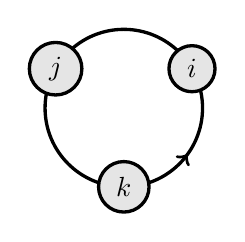
\begin{tikzpicture}[scale=1,very thick,decoration={
    markings,
    mark=at position 0.4 with {\arrow{>}}}
    ] 
  
  \draw[postaction={decorate}] (0:0)   circle (-1);
  \fill (30:1)  node[circle,draw,fill=black!10] {$i$}
        (150:1) node[circle,draw,fill=black!10] {$j$}
        (270:1) node[circle,draw,fill=black!10] {$k$};
\end{tikzpicture}
}
\end{center}
    
    \item An {\bf octonion} is an objects of the form $a+bi+cj+dk+el+fm+gn+ho$ with $a,\dots,h\in\mathbb{R}$ and $e_0=1, e_1=i, \dots, e_7=o$
    \begin{align}
        e_ie_j=\left\{\begin{array}{ll}
                e_j, & \text{if }i=0  \\
                e_i, & \text{if }j=0  \\
                -\delta_{ij}e_0 + \varepsilon_{ijk}e_k & \text{otherwise}
                \end{array}
                \right.
    \end{align}
\end{itemize}
\end{definition}

\begin{center}
\resizebox{2.5cm}{2cm}{
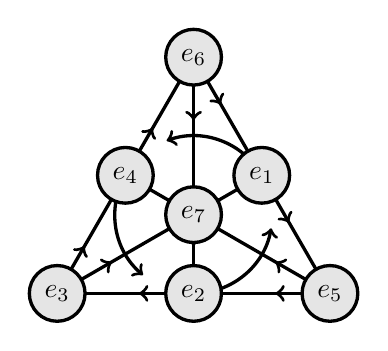
\begin{tikzpicture}[scale=1,very thick,decoration={
    markings,
    mark=at position 0.4 with {\arrow{>}}}
    ] 
  \draw[postaction={decorate}] (90:2)  --  (30:1);
  \draw[postaction={decorate}] (30:1)  --  (330:2);
  \draw[postaction={decorate}] (330:2)  --  (270:1);
  \draw[postaction={decorate}] (270:1)  --  (210:2);
  \draw[postaction={decorate}] (210:2)  --  (150:1);
  \draw[postaction={decorate}] (150:1)  --  (90:2);
  \draw[postaction={decorate}] (90:2)  --  (0:0);
  \draw[postaction={decorate}] (0:0)  --  (270:1);
  \draw[postaction={decorate}] (330:2)  --  (0:0);
  \draw[postaction={decorate}] (0:0)  --  (150:1);
  \draw[postaction={decorate}] (210:2)  --  (0:0);
  \draw[postaction={decorate}] (0:0)  --  (30:1);
  %\draw[postaction={decorate}] (0:0)   circle (-1);
  \draw[very thick, ->] (30:1) arc (30:110:1cm);
  \draw[very thick, ->] (270:1) arc (270:350:1cm);
  \draw[very thick, ->] (150:1) arc (150:230:1cm);
  
  \fill (0:0)   node[circle,draw,fill=black!10] {$e_7$}
        (30:1)  node[circle,draw,fill=black!10] {$e_1$}
        (90:2)  node[circle,draw,fill=black!10] {$e_6$}
        (150:1) node[circle,draw,fill=black!10] {$e_4$}
        (210:2) node[circle,draw,fill=black!10] {$e_3$}
        (270:1) node[circle,draw,fill=black!10] {$e_2$}
        (330:2) node[circle,draw,fill=black!10] {$e_5$};
\end{tikzpicture}
}
\end{center}

\begin{remark}{}
$\mathbb{C}$ forms a field, $\mathbb{H}$ forms a non-commutative ring
\end{remark}

\begin{definition}{}
The {\bf conjugates}  are defined by
\begin{align}
    \bar{z}&=a-bi\\
    \bar{q}&=a-bi-cj-dk\\
    &=-\frac{1}{2}\left[q+iqi+jqj+kqk\right]\\
    \bar x &= a-bi-cj-dk-el-fm-gn-ho\\
    &=-\frac{1}{6}\left[x+(ix)i+(jq)j+(kq)k)+(le)l+(mf)m+(ng)n+(oh)o\right]
\end{align}
\end{definition}

\subsection{Groups theory}
\begin{definition}{}
For a subgroup $H$ of a group $G$ {\bf a left-coset} of the subgroup $H$ in $G$ is defined as the set formed by a distinct $g\in G$
\begin{align}
    gH=\{gh: \forall h\in H\}
\end{align}
$G/H$ denotes the set of left cosets $\{gH: g \in G\}$ of $H$ in $G$ (called coset-space).
\end{definition}

\begin{definition}{}
A subgroup $N$ of a group $G$ is called {\bf normal subgroup (Normalteiler)} $N\vartriangleleft G$ if it is invariant under conjugation by members of $G$. Meaning
\begin{align}
    gng^{-1}\in N\quad \forall g\in G\\
    gN=Ng  \quad \forall g\in G\\
    gNg^{-1}=N  \quad \forall g\in G
\end{align}
\end{definition}

\begin{definition}{}
A {\bf simple group} is a nontrivial group whose only normal subgroups are the trivial group and the group itself.
\end{definition}

\begin{definition}{}
Let $(G,\circ)$ and $(K,*)$ be two groups with elements $g_a\in G$ and $k_i\in K$. The {\bf direct product} is a group $(G\otimes K,\star)$ with elements $(g_a,k_i)$ and the multiplication rule
\begin{align}
(g_a,k_i)\star(g_b,k_j)=(g_a\circ g_b,k_i*k_j).
\end{align}
\end{definition}

\begin{theorem}
Every finite simple group is isomorphic to one of the following groups:
\begin{enumerate}
    \item $Z_p$ cyclic group of prime order
    \item $A_n$ alternating group of degree $n>4$
    \item groups of Lie type (names derived from Lie algebras with $q=p^k, m\in\mathbb{N}$
    \begin{itemize}
        \item $A_n(q)$ Special projective linear group
        \item $B_n(q), n>1$ Commutator subgroup of $SO(2n+1)$ 
        \item $C_n(q), n>2$ projective symplectic group
        \item $D_n(q), n>1$ Commutator subgroup of $SO(2n)$ 
        \item $E_6(q), E_7(q), E_8(q), F_4(q), G_2(q)$ Chevalley group
        \item $^2A_n(q^2), n>1$ Special unitary group $SU(n)$
        \item $^2B_2(2^{2m+1}))$ Suzuki Groups $Sz(2^{2m+1})$
        \item $^2D_n(q^2), ^3D_4(q^3), ^2E_6(q^2)$ Steinberg group
        \item $^2F_4(2^{2m+1}), ^2G_2(2^{2m+1})$ Ree group
    \end{itemize}
    \item 26 sporadic groups
    \begin{itemize}
        \item Mathieu groups $M_{11}, M_{12}, M_{22}, M_{23}, M_{24}$
        \item Janko groups $J_1, J_2, J_3, J_4$
        \item Conway groups $Co_1, Co_2, Co_3$
        \item Fischer groups $Fi_{22}, Fi_{23}, F_{3+}$
        \item Higman–Sims group $HS$
        \item McLaughlin group $McL$
        \item Held group $F_7$
        \item Rudvalis group $Ru$
        \item Suzuki group $F_{3-}$
        \item O'Nan group $O'N$
        \item Harada–Norton group $F_5$
        \item Lyons group $Ly$
        \item Thompson group $F_3$
        \item Baby Monster group $F_2$
        \item Fischer–Griess Monster group $F_1$
    \end{itemize}
    \item $^2F_4(2)'$ Tits group (order $2^11\cdot3^3\cdot5^2\cdot13=17,971,200$)
    \begin{itemize}
        \item sometimes called the 27th sporadic group - but belongs for $m=0$ to the family $^2F_4(2^{2m+1})'$ of commutator subgroups of $^2F_4(2^{2m+1})$
    \end{itemize}
\end{enumerate}
\end{theorem}

\begin{figure}[htp]
    \centering
    %\includegraphics[width=8cm]{PTFSG.jpg}
    \caption{Periodic table of finite simple groups }
    \label{fig:galaxy}
\end{figure}

\begin{definition}{}
Exceptional Lie groups 
\begin{itemize}
    \item $G_2$ (order 14)
    \item $F_4$ (order 52)
    \item $E_6$ (order 78)
    \item $E_7$ (order 133)
    \item $E_8$ (order 248)
\end{itemize}
\end{definition}

\begin{theorem}
(Frobenius theorem, Hurwitz theorem) Any real finite-dimensional normed division algebra over the reals must be
\begin{itemize}
    \item isomorphic to $\mathbb{R}$ or $\mathbb{C}$ if unitary and commutative (equivalently: associative and commutative)
    \item isomorphic to the quaternions $\mathbb{H}$ if noncommutative but associative
    \item isomorphic to the octonions $\mathbb{O}$ if non-associative but alternative.
\end{itemize}
\end{theorem}


\begin{remark}{}
Projective spaces
\begin{itemize}
    \item $\mathfrak{so}(n+1)$ is infinitesimal isometry of the real projective spaces $\mathbb{RP}^n$
    \item $\mathfrak{su}(n+1)$ is infinitesimal isometry of the complex projective spaces $\mathbb{CP}^n$
    \item $\mathfrak{sp}(n+1)$ is infinitesimal isometry of the quaternionic projective spaces $\mathbb{HP}^n$
    \item octonionic projective line $\mathbb{OP}^1$ reproduces $\mathfrak{so}(8)$ (already accomodated by $\mathbb{RP}^7$)
    \item Cayley projective plane $\mathbb{OP}^2$ reproduces $\mathfrak{f}_4)$
    \item $\mathbb{OP}^n$ for $n>2$ gives nothing due to non-associativity of $\mathbb{O}$
\end{itemize}
\end{remark}

\begin{remark}{}
Freudenthal-Rosenfeld-Tits magic square of Lie algebras
\begin{align}
\begin{array}{c||cccc}
\mathbb{A}_1/\mathbb{A}_2 & \mathbb{R} & \mathbb{C} & \mathbb{H} & \mathbb{O}\\ \hline\hline
\mathbb{R} & \mathfrak{so}(3) & \mathfrak{su}(3) & \mathfrak{sp}(3) & \mathfrak{f}_4 \\
\mathbb{C} & \mathfrak{su}(3) & \mathfrak{su}(3)\otimes\mathfrak{su}(3) & \mathfrak{su}(6) & \mathfrak{e}_6  \\
\mathbb{H} & \mathfrak{sp}(3) & \mathfrak{su}(6) & \mathfrak{so}(12) & \mathfrak{e}_7  \\
\mathbb{O} & \mathfrak{f}_4   & \mathfrak{e}_6 & \mathfrak{e}_7& \mathfrak{e}_8 
\end{array}
\end{align}
\end{remark}



\subsection{Representation theory}
\theoremstyle{definition}
\begin{definition}{}
A {\bf representation} of a group $G=\left(\{g_i\},\circ\right)$ is a mapping $g\mapsto D(g)$ of the elements $g\in G$ onto a set of linear operators with
\begin{enumerate}
    \item $D(e)=\mathbb{I}$
    \item $D(g_1)D(g_2) = D(g_1\circ g_2)$.
\end{enumerate}
This obviously implies $D(g^{-1})=D(g)^{-1}$.
\end{definition}

\begin{remark}{}
A bit more formal - let $G$ a group and $V$ be a $\mathbb{K}$-vector space then a linear representation is a group homomorphism with
$D:G\rightarrow \GL(V)\overset{!}{=}\Aut(V)$. $V$ is then called representation space with $\dim V$ being the dimension of the representation and $D(g)\in\GL(V)$
\end{remark}

\begin{definition}{}
An {\bf equivalent representation} $D'$ of a representation $D$ is defined by 
\begin{align}
D(g)\rightarrow D'(g)=S^{-1}D(g)S   \qquad \forall g\in G
\end{align}
\end{definition}

\begin{definition}{}
A representation $D$ is called {\bf unitary representation} if 
\begin{align}
D(g)^\dagger=D(g)^{-1}    \qquad \forall g\in G
\end{align}
\end{definition}

\begin{remark}{}
For a unitary representation $D(g)^\dagger D(g)=\mathbb{I}$ an equivalent representation $D'(g)=S^{-1}D(g)S$ is only unitary
\begin{align}
    D'(g)^\dagger D'(g)&=\left(S^{-1}D(g)S\right)^\dagger S^{-1}D(g)S\\
    &=S^\dagger D(g)^\dagger (S^{-1})^\dagger S^{-1}D(g)S\\
    &=S^\dagger D(g)^\dagger (S^\dagger)^{-1} S^{-1}D(g)S\\
    &=S^\dagger D(g)^\dagger (SS^\dagger)^{-1} D(g)S
\end{align}
iff $S$ is unitary itself $SS^\dagger = \mathbb{I}$
\begin{align}
    D'(g)^\dagger D'(g)=S^{-1} D(g)^\dagger D(g)S = S^{-1} S = \mathbb{I}.
\end{align}
\end{remark}

\begin{definition}{}
A representation is called a {\bf reducible representation} if $V$ has an invariant subspace meaning that the action of any $D(g)$ on any vector of the subspace $V_P$ is still in the subspace. If the projection operator $P:V\rightarrow V_P$ projects to this subspace then
\begin{align}
PD(g)P=D(g)P   \qquad \forall g\in G
\end{align}
\end{definition}

\begin{remark}{}
$\forall |v\rangle\in V$ we have $P|v\rangle\in V_P$. If the subspace is invariant then any group action can not move it outside $D(g)P|v\rangle\in V_P$. But this means projecting it again would not change anything $PD(g)P|v\rangle = D(g)P|v\rangle$
\end{remark}

\begin{definition}{}
A representation is called an {\bf irreducible representation} if it is not reducible.
\end{definition}

\begin{definition}{}
A representation is called a {\bf completely reducible representation} if it is equivalent to a representation whose matrix elements have the form
\begin{align}
D(g)&=\left(
\begin{array}{ccc}
D_1(g) & 0      & \dots \\
0      & D_2(g) & \dots \\
\vdots & \vdots & \ddots
\end{array}
\right)
\end{align}
where all $D_j(g)$ are irreducible. Representation $D$ is is said to be the direct sum of subrepresentation $D_j$
\begin{align}
D&=D_1(g)\oplus D_2(g)\oplus\dotsi
\end{align}
\end{definition}

\begin{definition}{}
For a group of order $n$ the $n$-dimensional representation $D$ defined by 
\begin{align}
g_k&\rightarrow|e_k\rangle\\
D(g_j)|e_k\rangle&\overset{!}{=}|e_m\rangle\qquad\text{with } g_j\circ g_k=g_m\rightarrow|e_m\rangle
\end{align}
(where $\{|e_i\rangle\}$ is the ordinary $n$-dimensional cartesian basis) is called the {\bf regular representation}. The matrices are then constructed by
\begin{align}
[D(g_j)]_{ik}&=\langle e_i|D(g_j)|e_k\rangle=\langle e_i|e_m\rangle.
\end{align}
\end{definition}

\begin{theorem}
Every representation of a finite group is equivalent to a unitary representation.
\end{theorem}

\begin{theorem}
Every representation of a finite group is complete reducible.
\end{theorem}

\begin{definition}{}
Given two representations $D_1$ and $D_2$ acting on $V_1$ and $V_2$, an intertwiner between $D_1$ and $D_2$ is a linear operator $F:D_1\rightarrow D_2$ which ''commutes with $G$'' in the sense that
\begin{align}
F D_1(g) = D_2(g)F\quad \forall g \in G. 
\end{align}
\end{definition}



\chapter{Lie groups/algebras}
Linear representation
\begin{align}
g\to
\end{align}


\begin{remark}{}
Killing classification of simple Lie groups
\begin{itemize}
    \item SO(2n), SO(2n+1) - Lie algebra: $J^T=-J$ (skew-hermitian, trace free matrices $GL(n,\mathbb{R})$
    \item SU(n) - Lie algebra: $J^\dagger=-J$ (skew-hermitian, trace free matrices in $GL(n,\mathbb{C})$
    \item Sp(2n) - Lie algebra: $J^\dagger=-J$ (skew-hermitian matrices in $GL(n,\mathbb{H})$
\end{itemize}
\end{remark}

\chapter{Example representations}
\subsection{Cyclic group \texorpdfstring{$Z_2$}{TEXT}}
\begin{align}
\begin{array}{c||cc}
Z_2 & e & p \\ \hline\hline
e & e & p \\
p & p & e
\end{array}
\end{align}
\subsubsection{1d}
\begin{align}
D'(e)&=1,\quad D'(p)=-1
\end{align}

\subsection{Cyclic group \texorpdfstring{$Z_3$}{TEXT}}
\begin{align}
\begin{array}{c||ccc}
Z_3 & e & a & b \\ \hline\hline
e & e & a & b \\
a & a & b & e \\
b & b & e & a
\end{array}
\end{align}
\subsubsection{1d}
\begin{align}
D'(e)=1,\quad D'(a)=e^{i\frac{2\pi}{3}},\quad D'(b)=e^{i\frac{4\pi}{3}}
\end{align}


\subsubsection{3d - regular representation}
\begin{align}
|e\rangle=(1,0,0)^T,\quad |a\rangle=(0,1,0)^T,\quad |b\rangle=(0,0,1)^T
\end{align}
\begin{align}
D(e)=\left(\begin{array}{ccc}
1 & 0 & 0 \\
0 & 1 & 0 \\
0 & 0 & 1 
\end{array}
\right),\quad
D(a)=\left(\begin{array}{ccc}
0 & 0 & 1 \\
1 & 0 & 0 \\
0 & 1 & 0 
\end{array}
\right),\quad
D(b)=\left(\begin{array}{ccc}
0 & 1 & 0 \\
0 & 0 & 1 \\
1 & 0 & 0 
\end{array}
\right),\quad
\end{align}

\subsection{Dihedral group \texorpdfstring{$D_2=Z_2\otimes Z_2$}{TEXT}}
We construct the group table by utilizing the direct product rule
\begin{align}
(g_a,k_i)\star(g_b,k_j)=(g_a\circ g_b,k_i*k_j)
\end{align}
which simplifies to
\begin{align}
(g_a,g_i)\star(g_b,g_j)=(g_a\circ g_b,g_i\circ g_j).
\end{align}
\begin{align}
\begin{array}{c||cccc}
D_2   & (e,e) & (e,P) & (P,e) & (P,P) \\ \hline\hline
(e,e) & (e,e) & (e,P) & (P,e) & (P,P) \\
(e,P) & (e,P) & (e,e) & (P,P) & (P,e) \\
(P,e) & (P,e) & (P,P) & (e,e) & (e,P) \\
(P,P) & (P,P) & (P,e) & (e,P) & (e,e)
\end{array}
\end{align}


\subsection{Cyclic group \texorpdfstring{$Z_4$}{TEXT}}
\begin{align}
D'(e)=1,\quad 
D'(a)=e^{i\frac{1\pi}{4}},\quad 
D'(b)=e^{i\frac{2\pi}{4}},\quad 
D'(c)=e^{i\frac{3\pi}{4}}
\end{align}

\subsection{Group \texorpdfstring{$S_3$}{TEXT}}
\begin{align}
\begin{array}{c||cccccc}
S_3 & e   & a_1 & a_2 & a_3 & a_4 & a_5\\ \hline\hline
e   & e   & a_1 & a_2 & a_3 & a_4 & a_5\\
a_1 & a_1 & a_2 & e   & a_5 & a_3 & a_4 \\
a_2 & a_2 & e   & a_1 & a_4 & a_5 & a_3 \\
a_1 & a_3 & a_4 & a_5 & e   & a_1 & a_2 \\
a_1 & a_4 & a_5 & a_3 & a_2 & e   & a_1 \\
a_1 & a_5 & a_3 & a_4 & a_1 & a_2 & e \\
\end{array}
\end{align}
\begin{align}
a_1=(1,2,3),\quad a_2=(3,2,1),\quad a_3=(1,2),\quad a_4=(2,3),\quad a_5=(3, 1) 
\end{align}

\subsubsection{2d}
\begin{align}
D(e)=\left(\begin{array}{cc}
1 & 0\\
0 & 1
\end{array}
\right),\quad
D(a_1)=\left(\begin{array}{cc}
-\nicefrac{1}{2} & -\nicefrac{\sqrt{3}}{2}\\
 \nicefrac{\sqrt{3}}{2} & -\nicefrac{1}{2}
\end{array}
\right),\quad
D(a_2)=\left(\begin{array}{cc}
-\nicefrac{1}{2} & \nicefrac{\sqrt{3}}{2}\\
-\nicefrac{\sqrt{3}}{2} & -\nicefrac{1}{2}
\end{array}
\right),\\
D(a_3)=\left(\begin{array}{cc}
-1 & 0\\
0 & 1
\end{array}
\right),\quad
D(a_4)=\left(\begin{array}{cc}
\nicefrac{1}{2} & \nicefrac{\sqrt{3}}{2}\\
\nicefrac{\sqrt{3}}{2} & -\nicefrac{1}{2}
\end{array}
\right),\quad
D(a_5)=\left(\begin{array}{cc}
\nicefrac{1}{2} & -\nicefrac{\sqrt{3}}{2}\\
-\nicefrac{\sqrt{3}}{2} & -\nicefrac{1}{2}
\end{array}
\right)
\end{align}


\chapter{Resources}
\begin{itemize}


\item \href{https://ocw.mit.edu/courses/8-333-statistical-mechanics-i-statistical-mechanics-of-particles-fall-2013/video_galleries/video-lectures/}{Kardar - Statistical mechanics of particles}
\item \href{https://ocw.mit.edu/courses/8-334-statistical-mechanics-ii-statistical-physics-of-fields-spring-2014/video_galleries/video-lectures/}{Kardar - Statistical mechanics of fields}

\item \href{https://www.youtube.com/watch?v=seabT438nr0}{Nicolai - QFT}
\item \href{https://www.youtube.com/watch?v=EzfFklLqDjA&t=791s}{Luty - QFT}
\item \href{https://www.tpi.uni-jena.de/~floerchinger/qft1/Lecture01/}{Wetterich/Floechinger - QFT1}
\item \href{https://www.tpi.uni-jena.de/~floerchinger/qft2/lecture01/}{Wetterich/Floechinger - QFT2}
\item \href{https://www.youtube.com/@AlexFlournoyTeacher}{Flournoy QFT}
\item \href{https://www.youtube.com/watch?v=MqG-F6CV7qk&list=PLB6035BED574535DC}{Cahill - QFT 2011Spring}
\item \href{https://www.youtube.com/watch?v=Z4gC4ezAG0Y&list=PLpyIij4nP6QLfC2CsDF8CHzK6HkEkWCze}{Cahill QFT2 2019}
\item \href{https://www.youtube.com/playlist?list=PLpyIij4nP6QKgoKhAWKHZFHrvkFHsFZym}{Cahill QFT 2014}
\item \href{https://www.youtube.com/watch?v=0LWYXkeuy-Q}{Peskin - Standard Model}
\item \href{https://www.youtube.com/watch?v=Q3cHDiZIG44}{Bilal - Introduction to anomalies in QFT}
\item \href{https://www.youtube.com/@qftdominikstoeckinger1285/playlists}{Stoeckinger - QFT I/II/III}
\begin{enumerate}
\item Rel QFT WS19/20
\item Multiloop Renormalization WS20/21
\item Rel QFT 1B WS22/23
\item Rel QFT2 SS23
\item Standard Model SS23
\item Effective Field Theory SS24
\end{enumerate}

\item \href{https://www.youtube.com/playlist?list=PLAMDKMENB2xBOucbrZWja2Rs-SdqH7KIX}{Caltech Lectures on Geometric Methods in Physics}
\item \href{}{}

\item \href{https://www.youtube.com/watch?v=5IDHkKwXK4Y&list=PLaNkJORnlhZlAeFDKvWuoyqBBLPZ0F-3X}{Sorkin - Advanced course in GR (PI)}
\item \href{https://www.youtube.com/watch?v=IPxnAw91bMM&list=PLaNkJORnlhZkrH4w1AXqx4c4KNjJgh2rB}{Mukhanov - Advanded course in Cosmology (PI)}

\item \href{https://www.youtube.com/watch?v=3JhwuqEdyXM&list=PLaNkJORnlhZl6XY824eq9D2x6JoLwwpyr}{Perlick - Black holes}
\item \href{https://www.youtube.com/watch?v=Ssmr057FLEE}{Wald - Black hole Thermodynamics}

\item \href{https://ocw.mit.edu/courses/22-01-introduction-to-nuclear-engineering-and-ionizing-radiation-fall-2016/video_galleries/lecture-videos/}{Short - Introduction to nuclear engineering}

\item \href{https://www.arturekert.org/iqis}{Artur Ekert - Quantum Information}
\begin{itemize}
\item https://qubit.guide/index.html
\item https://www.youtube.com/@ArturEkert/playlists
\end{itemize}
\item \href{https://www.youtube.com/@StokesLine}{Complex Analysis}
\item \href{https://www.youtube.com/watch?v=VdLhQs_y_E8&list=PLelIK3uylPMGzHBuR3hLMHrYfMqWWsmx5}{Gross - Abstract algebra}
\item \href{https://www.maths.ed.ac.uk/~tl/gt/gt.pdf}{Leinster - Galois}
\item \href{http://www.math.toronto.edu/ivan/mat327/?resources}{Topology}
\item \href{https://www.youtube.com/watch?v=SXHHvoaSctc&list=PLTBqohhFNBE_09L0i-lf3fYXF5woAbrzJ}{Tokieda - Topology and Geometry}
\item Schiekel - Kruemmungen und Indexsaetze - auf den Spuren von Gauss-Bonnet, Cartan, Atiyah-Singer und Witten 3ed

\end{itemize}
\section{\href{https://www.youtube.com/@richarde.borcherds7998/playlists}{Richard Borcherds}}
\begin{enumerate}
\item Introduction to number theory (53)
\item Complex analysis (20)
\item Theory of numbers (20)
\item Zermelo Fraenkel axioms (8)
\item Group theory (32)
\item Rings and modules (22)
\item Galois theory (25)
\item Lie groups (11)
\item Representation theory (9)
\item Commutative Algebra (76)
\item Introduction to homological algebra (6)
\item Categories for the idle mathematician (7)
\item Modular forms (13)
\item Algebraic topology (4)
\item Algebraic geometry I: Varieties (51)
\item Algebraic geometry II: Schemes (48)
\item Algebraic geometry: Extra Topics (24)
\item Math talks (20)
\item History of science (7)
\end{enumerate}




\chapter{How to learn ...}
How to Learn Physics

big picture
\begin{itemize}
\item Emilio Segre, From Falling Bodies to Radio Waves: Classical Physicists and Their Discoveries, W. H. Freeman, New York, 1981.

\item Emilio Segre, From X-Rays to Quarks: Modern Physicists and Their Discoveries, W. H. Freeman, San Francisco, 1980.

\item Robert P. Crease and Charles C. Mann, The Second Creation: Makers of the Revolution in Twentieth-Century Physics, Rutgers University Press, New Brunswick, NJ, 1996.

\item Abraham Pais, Inward Bound: of Matter and Forces in the Physical World, Clarendon Press, New York, 1986. (More technical.)
Next, here are some good books to learn "the real stuff". These aren't "easy" books, but they're my favorites.
\end{itemize}

First, some very good general textbooks:
\begin{itemize}
\item M. S. Longair, Theoretical Concepts in Physics, Cambridge U. Press, Cambridge, 1986.

\item Richard Feynman, Robert B. Leighton and Matthew Sands, The Feynman Lectures on Physics, 3 volumes, Addison-Wesley, 1989. All three volumes are now free online.
\item Ian D. Lawrie, A Unified Grand Tour of Theoretical Physics, Adam Hilger, Bristol, 1990.
\end{itemize}

Classical mechanics:
\begin{itemize}
\item Herbert Goldstein, Charles Poole, and John Safko, Classical Mechanics, Addison Wesley, San Francisco, 2002.
\end{itemize}

Statistical mechanics:
\begin{itemize}
\item F. Reif, Fundamentals of Statistical and Thermal Physics, McGraw Hill, New York, 1965.
\end{itemize}

Electromagnetism:
\begin{itemize}
\item John David Jackson, Classical Electrodynamics, Wiley, New York, 1975.
\end{itemize}

Special relativity:
\begin{itemize}
\item Edwin F. Taylor, John A. Wheeler, Spacetime Physics: Introduction to Special Relativity, W. H. Freeman Press, 1992.
\end{itemize}

Quantum mechanics:
\begin{itemize}
\item Anthony Sudbery, Quantum Mechanics and the Particles of Nature: an Outline for Mathematicians, Cambridge University Press, Cambridge, 1986. (Not just for mathematicians!)

\item Claude Cohen-Tannoudji, Bernard Diu und Franck Laloë, Quantum Mechanics (2 volumes), Wiley-Interscience, 1992. 
\end{itemize}


General relativity — to get intuition for the subject before tackling the details:
\begin{itemize}
\item  Kip S. Thorne, Black Holes and Time Warps: Einstein's Outrageous Legacy, W. W. Norton, New York, 1994.
\item Robert M. Wald, Space, Time, and Gravity: the Theory of the Big Bang and Black Holes, University of Chicago Press, Chicago, 1977.
\item Robert Geroch, General Relativity from A to B, University of Chicago Press, Chicago, 1978.
\end{itemize}

General relativity — for when you get serious:
\begin{itemize}
\item  R. A. D'Inverno, Introducing Einstein's Relativity, Oxford University Press, Oxford, 1992.
\item J. B. Hartle, Gravity: An Introduction to Einstein's General Relativity, Addison-Wesley, New York, 2002.
\item B. F. Schutz, A First Course in General Relativity, Cambridge University Press, Cambridge, 1985.
\end{itemize}

General relativity — for when you get really serious:
\begin{itemize}
\item Charles W. Misner, Kip S. Thorne and John Archibald Wheeler, Gravitation, W. H. Freeman Press, San Francisco, 1973.
\item Robert M. Wald, General Relativity, University of Chicago Press, Chicago, 1984.
\end{itemize}

Cosmology:
\begin{itemize}
\item  Edward R. Harrison, Cosmology, the Science of the Universe, Cambridge University Press, Cambridge, 1981.
\item M. Berry, Cosmology and Gravitation, Adam Hilger, Bristol, 1986.
\item John A. Peacock, Cosmological Physics, Cambridge University Press, Cambridge, 1999. (More technical.)
\end{itemize}

Quantum field theory — to get intuition for the subject before tackling the details:
\begin{itemize}
\item  Richard Feynman, QED: the Strange Theory of Light and Matter, Princeton University Press, Princeton, 1985.
\end{itemize}

Quantum field theory — for when you get serious:
\begin{itemize}
\item  Michael E. Peskin and Daniel V. Schroeder, An Introduction to Quantum Field Theory, Addison-Wesley, New York, 1995. (The best modern textbook, in my opinion.)
\item A. Zee, Quantum Field Theory in a Nutshell, Princeton University Press, Princeton, 2003. (Packed with wisdom told in a charmingly informal manner; not the best way to learn how to calculate stuff.)
\item Warren Siegel, Fields, available for free on the arXiv.
\item Mark Srednicki, Quantum Field Theory, available free on his website. (It's good to snag free textbooks while you can, if they're not on the arXiv!)
\item Sidney Coleman, Physics 253: Quantum Field Theory, 1975-1976. (Not a book — it's a class! You can download free videos of this course at Harvard, taught by a brash and witty young genius.)
\end{itemize}

Quantum field theory — two classic older texts that cover a lot of material not found in Peskin and Schroeder's streamlined modern presentation:
\begin{itemize}
\item  James D. Bjorken and Sidney D. Drell, Relativistic Quantum Mechanics, New York, McGraw-Hill, 1964.
\item James D. Bjorken and Sidney D. Drell, Relativistic Quantum Fields, New York, McGraw-Hill, 1965.
\end{itemize}

Quantum field theory — for when you get really serious:
\begin{itemize}
\item  Sidney Coleman, Aspects of Symmetry, Cambridge U. Press, 1989. (A joy to read.)
\item Rudolf Haag, Local Quantum Physics: Fields, Particles, Algebras, Springer, 1992.
\end{itemize}

Quantum field theory — so even mathematicians can understand it:

\begin{itemize}
\item  Robin Ticciati, Quantum Field Theory for Mathematicians, Cambridge University Press, Cambridge, 1999.
\item Richard Borcherds and Alex Barnard, Lectures On Quantum Field Theory.
\end{itemize}

Particle physics:

\begin{itemize}
\item  Kerson Huang, Quarks, Leptons \& Gauge Fields, World Scientific, Singapore, 1982.
\item L. B. Okun, Leptons and Quarks, translated from Russian by V. I. Kisin, North-Holland, 1982. (Huang's book is better on mathematical aspects of gauge theory and topology; Okun's book is better on what we actually observe particles to do.)
\item T. D. Lee, Particle Physics and Introduction to Field Theory, Harwood, 1981.
\item K. Grotz and H. V. Klapdor, The Weak Interaction in Nuclear, Particle, and Astrophysics, Hilger, Bristol, 1990.
\end{itemize}


While studying general relativity and quantum field theory, you should take a break now and then and dip into this book: it's a wonderful guided tour of the world of math and physics:

\begin{itemize}
\item  Roger Penrose, The Road to Reality: A Complete Guide to the Laws of the Universe, Knopf, New York, 2005.
And then, some books on more advanced topics...
The interpretation of quantum mechanics:

\item Roland Omnes, Interpretation of Quantum Mechanics, Princeton U. Press, Princeton, 1994.
\end{itemize}

This is a reasonable treatment of an important but incredibly controversial topic. Warning: there's no way to understand the interpretation of quantum mechanics without also being able to solve quantum mechanics problems — to understand the theory, you need to be able to use it (and vice versa). If you don't heed this advice, you'll fall prey to all sorts of nonsense that's floating around out there.

The mathematical foundations of quantum physics:

\begin{itemize}
\item Josef M. Jauch, Foundations of Quantum Mechanics, Addison-Wesley, 1968. (Very thoughtful and literate. Get a taste of quantum logic.)

\item George Mackey, The Mathematical Foundations of Quantum Mechanics, Dover, New York, 1963. (Especially good for mathematicians who only know a little physics.)
\end{itemize}

Loop quantum gravity and spin foams:

\begin{itemize}
\item Carlo Rovelli, Quantum Gravity, Cambridge University Press, Cambridge, 2004.
String theory:

\item Barton Zwiebach, A First Course in String Theory, Cambridge U. Press, Cambridge, 2004. (The best easy introduction.)

\item Katrin Becker, Melanie Becker and John H. Schwartz, String Theory and M-Theory: A Modern Introduction, Cambridge U. Press, Cambridge, 2007. (A more detailed introduction.)

\item Michael B. Green, John H. Schwarz and Edward Witten, Superstring Theory (2 volumes), Cambridge U. Press, Cambridge, 1987. (The old testament.)

\item Joseph Polchinski, String Theory (2 volumes), Cambridge U. Press, Cambridge, 1998. (The new testament — he's got branes.)
\end{itemize}

How to Learn Math

Math is a much more diverse subject than physics, in a way: there are lots of branches you can learn without needing to know other branches first... though you only deeply understand a subject after you see how it relates to all the others!

The study of math branches out into a dizzying variety of more advanced topics! It's hard to get the "big picture" of mathematics until you've gone fairly far into it; indeed, the more I learn, the more I laugh at my previous pathetically naive ideas of what math is "all about". But if you want a glimpse, try these books:

\begin{itemize}
\item F. William Lawvere and Stephen H. Schanuel, Conceptual Mathematics: a First Introduction to Categories, Cambridge University Press, 1997. (A great place to start.)

\item Saunders Mac Lane, Mathematics, Form and Function, Springer, New York, 1986. (More advanced.)

\item Jean Dieudonne, A Panorama of Pure Mathematics, as seen by N. Bourbaki, translated by I.G. Macdonald, Academic Press, 1982. (Very advanced — best if you know a lot of math already. Beware: many people disagree with Bourbaki's outlook.)
\end{itemize}

I haven't decided on my favorite books on all the basic math topics, but here are a few. In this list I'm trying to pick the clearest books I know, not the deepest ones — you'll want to dig deeper later:

Finite mathematics (combinatorics):

\begin{itemize}
\item Arthur T. Benjamin and Jennifer Quinn, Proofs that Really Count: The Art of Combinatorial Proof, The Mathematical Association of America, 2003.

\item Ronald L. Graham, Donald Knuth, and Oren Patashnik, Concrete Mathematics, Addison-Wesley, Reading, Massachusetts, 1994. (Too advanced for a first course in finite mathematics, but this book is fun — quirky, full of jokes, it'll teach you tricks for counting stuff that will blow your friends minds!)
\end{itemize}

Probability theory:

\begin{itemize}
\item Charles M. Grinstead and J. Laurie Snell, Introduction to Probability, American Mathematical Society, Providence, Rhode Island, 1997. Also available free online at https://math.dartmouth.edu/~prob/prob/prob.pdf.
\end{itemize}

Calculus:

\begin{itemize}
\item Silvanus P. Thompson, Calculus Made Easy, St. Martin's Press, 1914. Also available free online at http://www.gutenberg.org/ebooks/33283. (Most college calculus texts weigh a ton; this one does not — it just gets to the point. This is how I learned calculus: my uncle gave me a copy.)

\item Gilbert Strang, Calculus, Wellesley-Cambridge Press, Cambridge, 1991. Also available free online at http://ocw.mit.edu/ans7870/resources/Strang/strangtext.htm. (Another classic, with lots of applications to real-world problems.)
\end{itemize}

Multivariable calculus:

\begin{itemize}
\item James Nearing, Mathematical Tools for Physics, available at http://www.physics.miami.edu/~nearing/mathmethods/. See especially the sections on multvariable calculus, vector calculus 1, and vector calculus 2. (Very nice explanations!)

\item George Cain and James Herod, Multivariable Calculus. Available free online at http://www.math.gatech.edu/~cain/notes/calculus.html
\end{itemize}

Linear algebra:

This is a great linear algebra book if you want to understand the subject thoroughly:

\begin{itemize}
\item Elizabeth S. Meckes and Mark Meckes, Linear Algebra, Cambridge U. Press, 2018.

These books are probably easier, and they're free online:

\item Keith Matthews, Elementary Linear Algebra, available free online at http://www.numbertheory.org/book/.

\item Jim Hefferon, Linear Algebra, available free online at http://joshua.smcvt.edu/linalg.html/.

\item Robert A. Beezer, A First Course in Linear Algebra, available free online at http://linear.ups.edu/.
\end{itemize}

Ordinary differential equations — some free online books:

\begin{itemize}
\item Bob Terrell, Notes on Differential Equations, available free online at http://www.math.cornell.edu/~bterrell/dn.pdf. (Does both ordinary and partial differential equations.)

\item James Nearing, Mathematical Tools for Physics, available at http://www.physics.miami.edu/~nearing/mathmethods/. See especially the sections on ordinary differential equations and Fourier series (which are good for solving such equations).
\end{itemize}

Partial differential equations — some free online books:

\begin{itemize}
\item Bob Terrell, Notes on Differential Equations, available free online at http://www.math.cornell.edu/~bterrell/dn.pdf. (Does both ordinary and partial differential equations.)

\item James Nearing, Mathematical Tools for Physics, available at http://www.physics.miami.edu/~nearing/mathmethods/. See especially the section on partial differential equations.
\end{itemize}

Set theory and logic:

\begin{itemize}
\item Herbert B. Enderton, Elements of Set Theory, Academic Press, New York, 1977.

\item Herbert B. Enderton, A Mathematical Introduction to Logic, Academic Press, New York, 2000.

\item F. William Lawvere and Robert Rosebrugh, Sets for Mathematics, Cambridge U. Press, Cambridge, 2002. (An unorthodox choice, since this book takes an approach based on category theory instead of the old-fashioned Zermelo-Fraenkel axioms. But this is the wave of the future, so you might as well hop on now!)
\end{itemize}

Complex analysis:

\begin{itemize}
\item George Cain, Complex Analysis, available free online at http://www.math.gatech.edu/~cain/winter99/complex.html. (How can you not like free online?)

\item James Ward Brown and Ruel V. Churchill, Complex Variables and Applications, McGraw-Hill, New York, 2003. (A practical introduction to complex analysis.)

\item Serge Lang, Complex Analysis, Springer, Berlin, 1999. (More advanced.)
\end{itemize}

Real analysis:

\begin{itemize}
\item  Richard R. Goldberg, Methods of Real Analysis, Wiley, New York, 1976. (A gentle introduction.)

\item Halsey L. Royden, Real Analysis, Prentice Hall, New York, 1988. (A bit more deep; here you get Lebesgue integration and measure spaces.)
\end{itemize}

Topology:

\begin{itemize}
\item  James R. Munkres, Topology, James R. Munkres, Prentice Hall, New York, 1999.

\item Lynn Arthur Steen and J. Arthur Seebach, Jr., Counterexamples in Topology, Dover, New York, 1995. (It's fun to see how crazy topological spaces can get: also, counterexamples help you understand definitions and theorems. But, don't get fooled into thinking this stuff is the point of topology!)
\end{itemize}

Abstract algebra:

I didn't like abstract algebra as an undergrad. Now I love it! Textbooks that seem pleasant now seemed dry as dust back then. So, I'm not confident that I could recommend an all-around textbook on algebra that my earlier self would have enjoyed. But, I would have liked these:

\begin{itemize}
\item Hermann Weyl, Symmetry, Princeton University Press, Princeton, New Jersey, 1983. (Before diving into group theory, find out why it's fun.)

\item Ian Stewart, Galois Theory, 3rd edition, Chapman and Hall, New York, 2004. (A fun-filled introduction to a wonderful application of group theory that's often explained very badly.)
\end{itemize}

Number theory:

These are elementary textbooks; for more advanced ones read on further.

\begin{itemize}
\item George E. Andews, Number Theory, Dover, New York, 1994. (A good elementary introduction; don't buy the Kindle version of this edition since the equations are tiny.)
\item Joseph Silverman, Friendly Introduction to Number Theory, Pearson, 2017. (Doesn't require any advanced mathematics, not even calculus.)
\item Martin H. Weissman, An Illustrated Theory of Numbers, American Mathematical Society, Providence, Rhode Island, 2017. (This reveals the oft-hidden visual side of number theory.)
\end{itemize}

More Advanced Math

I'll start with some books on mathematical physics, because that's been one of my favorite subjects for a long time. Out of laziness, I'll assume you're already somewhat comfortable with the topics listed above — yes, I know that requires about 4 years of full-time work! —l and I'll pick up from there. Here's a good place to start:

\begin{itemize}
\item Paul Bamberg and Shlomo Sternberg, A Course of Mathematics for Students of Physics, Cambridge University, Cambridge, 1982. (A good basic introduction to modern math, actually.)

It's also good to get ahold of these books and keep referring to them as needed:

\item Robert Geroch, Mathematical Physics, University of Chicago Press, Chicago, 1985.
\item Yvonne Choquet-Bruhat, Cecile DeWitt-Morette, and Margaret Dillard-Bleick, Analysis, Manifolds, and Physics (2 volumes), North-Holland, 1982 and 1989.

Here's a free online reference book that's 787 pages long:

\item Jean Claude Dutailly, Mathematics for Theoretical Physics, 2012.
\end{itemize}

Here are my favorite books on various special topics:

Group theory in physics:

\begin{itemize}
\item Shlomo Sternberg, Group Theory and Physics, Cambridge University Press, 1994.
\item Robert Hermann, Lie Groups for Physicists, Benjamin-Cummings, 1966.
\item George Mackey, Unitary Group Representations in Physics, Probability, and Number Theory, Addison-Wesley, Redwood City, California, 1989.
\end{itemize}

Lie groups, Lie algebras and their representations — in rough order of increasing sophistication:

\begin{itemize}
\item Brian Hall, Lie Groups, Lie Algebras, and Representations, Springer, Berlin, 2003.
\item William Fulton and Joe Harris, Representation Theory — a First Course, Springer, Berlin, 1991. (A friendly introduction to finite groups, Lie groups, Lie algebras and their representations, including the classification of simple Lie algebras. One great thing is that it has many pictures of root systems, and works slowly up a ladder of examples of these before blasting the reader with abstract generalities.)
\item J. Frank Adams, Lectures on Lie Groups, University of Chicago Press, Chicago, 2004. (A very elegant introduction to the theory of semisimple Lie groups and their representations, without the morass of notation that tends to plague this subject. But it's a bit terse, so you may need to look at other books to see what's really going on in here!)
\item Daniel Bump, Lie Groups, Springer, Berlin, 2004. (A friendly tour of the vast and fascinating panorama of mathematics surrounding groups, starting from really basic stuff and working on up to advanced topics. The nice thing is that it explains stuff without feeling the need to prove every statement, so it can cover more territory.)
\end{itemize}

Geometry and topology for physicists — in rough order of increasing sophistication:

\begin{itemize}
\item Gregory L. Naber, Topology, Geometry and Gauge Fields: Foundations, Springer, Berlin, 1997.
\item Chris Isham, Modern Differential Geometry for Physicists, World Scientific Press, Singapore, 1999. (Isham is an expert on general relativity so this is especially good if you want to study that.)
\item Harley Flanders, Differential Forms with Applications to the Physical Sciences, Dover, New York, 1989. (Everyone has to learn differential forms eventually, and this is a pretty good place to do it.)
\item Charles Nash and Siddhartha Sen, Topology and Geometry for Physicists, Academic Press, 1983. (This emphasizes the physics motivations... it's not quite as precise at points.)
\item Mikio Nakahara, Geometry, Topology, and Physics, A. Hilger, New York, 1990. (More advanced.)
\item Charles Nash, Differential Topology and Quantum Field Theory, Academic Press, 1991. (Still more advanced — essential if you want to understand what Witten is up to.)
\end{itemize}

Geometry and topology, straight up:

\begin{itemize}
\item Victor Guillemin and Alan Pollack, Differential Topology, Prentice-Hall, Englewood Cliffs, 1974.
\item B. A. Dubrovin, A. T. Fomenko, and S. P. Novikov, Modern Geometry — Methods and Applications, 3 volumes, Springer, Berlin, 1990. (Lots of examples, great for building intuition, some mistakes here and there. The third volume is an excellent course on algebraic topology from a geometrical viewpoint.)
\end{itemize}

Algebraic topology:

\begin{itemize}
\item Allen Hatcher, Algebraic Topology, Cambridge U. Press, Cambridge, 2002. Also available free at http://www.math.cornell.edu/~hatcher/AT/ATpage.html. (An excellent modern introduction.)
\item Peter May, A Concise Course in Algebraic Topology, U. of Chicago Press, Chicago, 1999. Also available free at http://www.math.uchicago.edu/~may/CONCISE/ConciseRevised.pdf. (More intense.)
\end{itemize}

Geometrical aspects of classical mechanics:

\begin{itemize}
\item Vladimir I. Arnol'd, Mathematical Methods of Classical Mechanics, translated by K. Vogtmann and A. Weinstein, 2nd edition, Springer, Berlin, 1989. (The appendices are somewhat more advanced and cover all sorts of nifty topics.)
\end{itemize}

Analysis and its applications to quantum physics:

\begin{itemize}
\item Michael Reed and Barry Simon, Methods of Modern Mathematical Physics (4 volumes), Academic Press, 1980.
\end{itemize}

And moving on to pure mathematics...
Knot theory:

\begin{itemize}
\item Louis Kauffman, On Knots, Princeton U. Press, Princeton, 1987.
\item Louis Kauffman, Knots and Physics, World Scientific, Singapore, 1991.
\item Dale Rolfsen, Knots and Links, Publish or Perish, Berkeley, 1976.
\end{itemize}

Homological algebra:

\begin{itemize}
\item Joseph Rotman, An Introduction to Homological Algebra, Academic Press, New York, 1979. (A good introduction to an important but sometimes intimidating branch of math.)

\item Charles Weibel, An Introduction to Homological Algebra, Cambridge U. Press, Cambridge, 1994. (Despite having the same title as the previous book, this goes into many more advanced topics.)
\end{itemize}

Combinatorics:

\begin{itemize}
\item Herbert Wilf, Generatinfunctionology, Academic Press, 1994. (Tons of fun and also available free online at https://www.math.upenn.edu/~wilf/DownldGF.html. It's good to read this after Concrete Mathematics by Graham, Knuth and Pataschnik, listed above under combinatorics.)
\item Richard P. Stanley, Enumerative Combinatorics, two volumes, Cambridge U. Press, 1997. (Packed with great exercises; volume one is also available free online at http://www-math.mit.edu/~rstan/ec/ec1.pdf.)
\end{itemize}

Algebraic geometry:

I found Hartshorne's famous book quite off-putting the first ten times I tried to read it. I think it's better to start by getting to know some 'classical' algebraic geometry so you see why the subject is interesting and why it's called 'geometry' before moving on to delightful modern abstractions like schemes. So, start with this introduction:

\begin{itemize}
\item Karen E. Smith, Lauri Kahanpää, Pekka Kekäläinen and William Traves, An Invitation to Algebraic Geometry, Springer, Berlin, 2004.

Then try these:

\item Igor R. Shafarevich, Basic Algebraic Geometry, two volumes, third edition, Springer, 2013.
\item David Eisenbud and Joseph Harris, The Geometry of Schemes, Springer, 2006.
\item Phillip Griffiths and Joseph Harris, Principles of Algebraic Geometry, 1994. (Especially nice if you like complex analysis, differential geometry and de Rham theory.)
\end{itemize}

Number theory:

\begin{itemize}
\item Kenneth Ireland and Keith Rosen, A Classical Introduction to Modern Number Theory, second edition, Springer, 1998. (A good way to catch up on some classic results in number theory while getting a taste of modern methods.)
\item Yu. I. Manin and Alexei A. Panchishkin, Introduction to Modern Number Theory: Fundamental Problems, Ideas and Theories, Springer, 2007. (Much more hard-hitting, but a very useful overview of what modern number theory is like.)
\item Jürgen Neukirch, Algebraic Number Theory, Springer, 2010. (A friendly introduction to class field theory.)
\end{itemize}
Category theory:

\begin{itemize}
\item Brendan Fong and David Spivak, Seven Sketches in Compositionality: An Invitation to Applied Category Theory. (A good first introduction to category theory through applications; available free online at http://math.mit.edu/~dspivak/teaching/sp18/7Sketches.pdf. Also see the website with videos and my online course based on this book.)
\item Tom Leinster, Basic Category Theory, Cambridge Studies in Advanced Mathematics, Vol. 143, Cambridge U. Press, 2014. Also available for free on the arXiv. (A introduction for beginners that focuses on three key concepts and how they're related: adjoint functor, representable functors, and limits.)
\item Emily Riehl, Category Theory in Context, Dover, New York, 2016. Also available for free on her website. (More advanced. As the title suggests, this gives many examples of how category theory is applied to other subjects in math.)
\end{itemize}

\newpage
In this section, I discuss some books that
\begin{enumerate}
\item discuss the mathematical background for GR (differential geometry),
\item place relativity theory in the context of physics at large,
\item contain important milestones in the history of relativity theory.
\end{enumerate}

I'll begin with several books in the Schaum's outline series, which, if read with discipline, can actually be a very effective way, I think, to learn some problem-solving skills.  If you really are starting with linear algebra, however, you should expect to spend many months in hard labor working through these books before you are ready to being your study of GR.  I am not familiar with all of the following books, but consider the one I own (the last) to be a good book.

\begin{itemize}
\item Seymour Lipschutz,
Schaum's Outline of Linear Algebra, 2nd ed.
McGraw-Hill, 1991.
In print, ISBN 0-07-038007-4; list price 13.95 (paperback).

\item Frank Ayres and Elliot Mendelson,
Schaum's Outline of Calculus, 3rd ed.
McGraw-Hill, 1990.
In print, ISBN 0-07-002662-9; list price 14.95 (paperback).

\item Richard Bronson,
Schaum's Outline of Differential Equations, 2nd ed.
McGraw-Hill, 1994.
In print, ISBN 0-07-008019-4; list price 14.95 (paperback).

\item Paul C. DuChateau, and D. W. Zachmann,
Schaum's Outline of Partial Differential Equations
McGraw-Hill, 1986.
In print, ISBN 0-07-017897-6; list price 14.95 (paperback).

\item Murray R. Spiegel,
Advanced Mathematics for Engineers and Scientists.
McGraw-Hill, 1971.
In print, ISBN 0-07-060216-6; list price 14.95 (paperback).

\item Martin Lipschutz,
Differential Geometry.
McGraw-Hill, 1969.
In print, ISBN 0-07-037985-8; list price 12.95 (paperback).
\end{itemize}

A good introduction to classical differential geometry.  Note well; for GR you need more advanced notions, including modern notions of manifolds, covariant, Lie, and exterior derivatives, connections, and curvature tensors.

\begin{itemize}
\item David C. Kay,
Schaum's Outline of Tensor Calculus
McGraw-Hill, 1988.
In print, ISBN 0-07-033484-6; list price

An introduction to coordinate basis tensor computations, including the metric tensor, geodesics, the Riemann tensor, with applications to classical mechanics and SR (but not GR).  This won't entirely get you up to speed for GR, but like the previous book it may be useful as a supplementary text.

\item John H. Hubbard,
Vector Calculus, Linear Algebra and Differential Forms: A Unified Approach.
Prentice Hall, 1998.
In print, ISBN 0-13-657446-7; 

This book can probably serve as a substitute for all of the Schaum's books mentioned above (save the last two), with the additional bonus of introducing exterior forms early on and properly emphasizing the fact that these objects are natural, easy to understand, and easy to compute with.

\item Theodore Frankel,
The Geometry of Physics: An Introduction.
Cambridge University Press, 1997.
In print, ISBN 0-521-38334-X; 

This book is simply gorgeous.  It offers a thorough and beautifully illustrated introduction to everything from riemannian geometry, Cartan geometry, symplectic geometry, differential topology and Morse Theory to vector bundles and Pontryagin and Chern classes.  Applications to hamiltonian mechanics, GR, Yang-Mills theories, the Standard Model of particle physics, etc., are also sketched.
\end{itemize}



Speaking of manifolds and differential geometry, I think that one of the best all around introductions is:

\begin{itemize}
\item William M. Boothby,
An Introduction to Differentiable Manifolds and Riemannian Geometry, 2nd ed.
Academic Press, 1986.
In print, ISBN 0-12-116053-X;.

One book which is particularly well suited for background reading in GR is the outrageously expensive

\item Barrett O'Neill,
Semi-Riemannian Geometry with Applications to Relativity.
Academic Press, 1983.
In print, ISBN 0-12-526740-1; 

This book covers not only manifolds, tensors, metrics, connections, curvature, calculus of variations, homogeneous spaces, and covering spaces, but also Minkowski spacetime, the Friedmann and Schwarzschild solutions, and the singularity theorems.

Another classic, easy to read introduction is "the great American differential geometry book":

\item Michael Spivak,
A Comprehensive Introduction to Differential Geometry, 5 volumes. Publish or Perish, 1979.
\begin{enumerate}
\item Vol.: ISBN 0-914098-84-5; 
\item Vol.: ISBN 0-914098-85-3;
\item Vol.: ISBN 0-914098-86-1;
\item Vol.: ISBN 0-914098-87-X;
\item Vol.: ISBN 0-914098-88-8; (all in hardcover only).
\end{enumerate}

This book has a somewhat fussy notation, and tends toward the verbose, but it is engaging and full of insight.  Boothby is shorter but covers more, although the last volume of Spivak is a gentle introduction to Chern classes.

A gentle introduction by popular author is:

\item Frank Morgan,
Riemannian Geometry: A Beginner's Guide, 2nd ed.
A K Peters, 1997.
In print, ISBN 1-56881-073-3; 

Another well known textbook (the author is a relativist) is:

\item Barrett O'Neill,
Elementary Differential Geometry, 2nd ed.
Academic Press, 1997.
In print, ISBN 0-12-526745-2; list price 49.95 (hardcover).

Another well known textbook (aimed more at hamiltonian mechanics) is:

\item R. Abraham, Jerrold E. Marsden, and T. Ratiu,
Manifolds, Tensor Analysis, and Applications.
Springer-Verlag, 1996.
In print, ISBN 0-387-96790-7; list price 69.95 (hardcover).

A cheaper alternative is:

\item Richard Bishop and Samuel Goldberg,
Tensor Analysis on Manifolds.
Dover, 1980.
In print, ISBN 0-486-64039-6; list price 8.95 (paperback).

At a higher level, try:

\item Y. Choquet-Bruhat, C. DeWitt-Morette, and M. Dillard-Bleick,
Analysis, Manifolds and Physics, Pt. I: Basics.  Revised ed.
Elsevier Science, 1991.
In print, ISBN 0-444-86017-7; list price 63.50 (paperback).
Note that the first author has made important contributions to GR.

The most influential geometry book of all time is:

\item Shoshichi Kobayashi and Katsumi Nobizu,
Foundations of Differential Geometry.  Two volumes.
John Wiley \& Sons, 1996.
In print, ISBN 0-471-15733-3; list price 59.95 (paperback).
Not for the faint of heart.

A textbook by the greatest geometer of all time is:

\item Shiing-Shen Chern,
Differential Geometry.
World Scientific, 1998.
In print, ISBN 981-02-2647-0; list price 26.00 (paperback).
For the Russian perspective (one author is a legendary relativist), try:

\item B. A. Dubrovin, A. T. Fomenko, and S. P. Novikov,
Modern Geometry - Methods and Applications.  2 volumes, 2nd ed.
Springer-Verlag, 1993.
In print, ISBN 0-387-97663-9; list price 65.9a (hardcover).

I am not familiar with the following book, but I like an elementary GR text by the second author:

\item F. De Felice, C. J. Clarke,
Relativity on Curved Manifolds.
Cambridge University Press, 1992.
ISBN 0-521-42908-0; list price 42.95 (paperback).
Here are two pricey and extremely concise outlines of the basics of differential geometry and topology as they are used in modern physics:

\item M. Nakahara,
Geometry, Topology and Physics.
I O P Publishing, 1990.
In print, ISBN 0-85274-095-6; list price 61.00 (paperback).

\item Charles Nash and Siddartha Sen.
Topology and Geometry for Physicists.
Academic Press, 1988 (reprint).

In print, ISBN 0-12-514081-9; list price 58.00 (paperback).
These are so dense I wouldn't recommend them for anyone without a strong background in modern physics.

Dover has reprinted books by Levi-Civita, Schouten, and Synge on tensor calculus.  These were all essential references in their day but they are now hopelessly out of date and I recommend that students spend their money on more expensive but more modern texts.

Here are some books that may help the student place relativity theory into the grand scheme of things, physically speaking:

\item I.D. Lawrie,
A Unified Grand Tour of Theoretical Physics.
I O P Publishing, 1990.
In print, ISBN 0-85274-015-8; list price 49.00 (paperback).
I like this book very much.  Lawrie quite properly emphasizes the formal analogies between hamiltonian mechanics and quantum theory; the variational principle formulations of GR ties this relativity theory to both these subjects.  Lawrie also emphasizes the fact that newtonian theory is not simply "wrong"; by a mere change of interpretation (and a factor of i here and a factor of h bar there) the equations of newtonian theory (as rewritten by Hamilton) go over to their quantum analogs.  Needless to say these formal analogies are a great help to the working physicist.

\item Richard P. Feynman,
The Feynman Lectures on Physics
Addison Wesley Longman, 1970.  3 Volumes.
In print, available as boxed set or individual paperbacks.

One of the great scientific expositions of all time.  Full of enthusiasm and overflowing with fabulous ideas.  Feynman's geometric explanation of the physical meaning of Maxwell's equation is a joy; so is his discussion of action at a distance (his revolutionary work with Wheeler).  The first two volumes are particularly recommended.  Note well: in volume 2, the section on SR is one of the few weak points in the book; I advise that you skip it altogether.  If you must read it, not, RPF is not saying that spacetime has a Euclidean metric!

\item L. D. Landau, E. M. Lifshitz and others,
Course of Theoretical Physics, 8 volumes.
Butterworth-Heinemann, various years.

Vol. 1 (Mechanics) and Vol. 2 (Classical Field Theory) are particularly relevant.  Well translated and quite readable for the most part.  Initiated by the great Russian physicist Lev Landau and continued after his untimely death by his disciple Lifshitz.  The Russian approach to physics and math is significantly different from American ideas in many respects and it is worthwhile gaining some familiarity with Landau's vision.  Unlike say Feynman's great books, this series offers many excellent exercises.

\item Walter Greiner and others.
A Curriculum in Theoretical Physics.
Springer-Verlag, various years.
Another heroic attempt to survey all of modern theoretical physics at the advanced undergraduate to second year graduate level, this time with a European perspective.  Well translated from the German, very readable, with an excellent balance of theory, descriptions of "great experiments", and practical experience in computing things using the theory.  Many exercises are solved in full.

Here are some books that relate relativity theory to important subjects in mathematics:

\item E. J. Flaherty,
Hermitian and Kahlerian Geometry in Relativity.
Springer-Verlag New York, 1976.
Out of print.

In Kahler geometry, instead of bundling tangent planes with a euclidean inner product, we bundle tangent planes with a hermitian inner product, which gives a much more "rigid" structure.  But symplectic geometry may be even more important in the future; see

\item M. Kauderer,
Symplectic Matrices, First Order Systems and Special Relativity.
World Scientific, 1994.
In print, ISBN 981-02-0829-4; list price 64.00 (hardcover).

\item Victor W. Guillemin and Shlomo Sternberg,
Symplectic Techniques in Physics.
Cambridge University Press, 1990.
In print, ISBN 0-521-38990-9; list price 37.95 (paper).

\item Helmut Hofer and Eduard Zehnder,
Symplectic Invariants and Hamiltonian Dynamics.
Birkhauser, 1994.
In print, ISBN 0-8176-5066-0; list price 59.50 (hardcover).

\item J. M. Souriau,
Structure of Dynamical Systems: A Symplectic View of Physics.
Birkhauser, 1997.
Out of print.

\item Dusa McDuff and Dietmar Salamon,
Introduction to Symplectic Topology.
Oxford University Press, 1995.
In print, ISBN 0-19-851177-9; list price 90.00 (hardcover).

\item A. T. Fomenko,
Symplectic Geometry, 2nd ed.
Gordon \& Breach Publishing Group, 1995.
In print, ISBN 2-88124-901-9; list price 110.00 (hardcover).

Finally, for a glimpse of what quantum gravity may look like, try:

\item J. Baez and J. Muniain,
Gauge Fields, Knots and Gravity.
World Scientific, 1994.
In print, ISBN 981-02-2034-0; list price 43.00 (paperback).

This book also features an excellent and concise introduction to exterior forms and a good discussion of the rather vexed terms "contravariant" and "covariant" (they way they are used in older GR books is exactly opposite to their modern meaning in mathematics!) [From the editor (DK): But I think their use in older books makes much more sense!]

Here are some books of enduring historical interest:

\item Albert Einstein and others,
The Principle of Relativity
Dover, 1952 reprint.
In print, ISBN 0-486-60081-5; list price 7.95 (paperback).

A collection of historic papers by Lorentz, Einstein, and others, including Einstein's 1905 paper on STR, his 1907 paper on the equivalence of mass and energy, Minkowski's 1908 paper introducing the physical interpretation of his geometry, Einstein's 1916 paper on the foundations of GTR, and early attempts to unify EM and gravitation.  In particular, the paper by Weyl laid the foundation for Yang-Mills theories, and the paper by Kaluza and Klein contains the idea of "compactified dimensions" which is a key element of modern string theories.

\item Hermann Weyl,
Space, Time, Matter
Dover, 1922.
In print, ISBN 0-486-60267-2; list price 9.95 (paperback).

Weyl was one of the great mathematicians of the early twentieth century, and one of the first to appreciate the importance of Einstein's ideas about gravitation and unified field theories.  In this quirky but clearly written book, he describes the five year old theory of GR, assuming virtually no mathematical prerequisites, and attempts to go beyond it with ideas on non-riemannian connections which were several generations ahead of their time (in terms of physical application).

\item Richard C. Tolman,
Relativity, Thermodynamics and Cosmology
Dover, 1987 reprint.
In print, ISBN 0-486-65383-8; list price 13.95 (paperback).

An important resource in the thirties and forties but by now hopelessly out of date.

\item Arthur S. Eddington,
Space, Time and Gravitation: An Outline of the General Theory.
Cambridge University Press, 1987.
In print, ISBN 0-521-33709-7; list price 24.95 (paperback).

A classic semipopular book, by now hopelessly outdated, but written with the engaging, stylish verve that made Eddington one of the most popular science writers of his day.

\item Wolfgang Pauli,
Theory of Relativity.
Dover, 1981 reprint.
In print, ISBN 0-486-64152-X; list price 8.95 (paperback).

This was the first book on relativity theory, written in a burst of youthful enthusiasm by the twenty year old Pauli.  Needless to say, it is of purely historical interest today.

Here is a book which is quirky but which will be valuable to some readers:

\item Richard P. Feynman,
Lectures on Gravitation.
Addison Wesley Longman, 1995.
In print, ISBN 0-201-62734-5; list price 38.43 (hardcover).

Feynman's attempt to motivate the field equation "in the spirit of QFT"; this approach is somewhat similar to that adopted in Ohanian et al., but this book is of interest mainly for watching Feynman at play.
\end{itemize}


Histories, Biographies, and Memoirs

\begin{itemize}
\item Abraham Pais,
Subtle Is the Lord: The Science and Life of Albert Einstein
Oxford University Press, 1983.
In print, ISBN 0-19-520438-7, list price 17.95 (paperback)

This is the definitive scientific biography, written a noted physicist who personally knew Einstein, Bohr, and other key people in AE's career, and who has read every paper AE ever wrote.  Features a fascinating, detailed—and fully technical—account of Einstein's heroic struggle toward his field equations.

\item Roberto Torretti,
Relativity and Geometry
Dover, 1996 (reprint).
In print, ISBN 0-486-69046-6; list price 14.95 (paperback).
This is another scientific biography focusing on the work rather than the man, offering some mathematical commentary on Einstein's struggle toward the field equation, and also discussing Einstein's "philosophy".

\item Don Howard and John J. Stachel,
Einstein: The Formative Years, 1879-1909
Birkhauser, 1998.
In print, ISBN 3-7643-4030-4, (price not available).

Another recent biography of Einstein.

\item John A. Wheeler and Kenneth Ford,
Geons, Black Holes, and Quantum Foam: A Life in Physics
W. W. Norton \& Company, 1998.
In print, ISBN 0-393-04642-7, list price 27.95 (hardcover).
The autobiography of the physicist widely credited (along with Subrahmanyan Chandrasekhar) with transforming the notion of a black hole from dubious speculation into a common, and in some ways, quite well understood natural object.

The book by Kip Thorne (a former PhD student of Wheeler, who has had a distinguished career in his own right) cited above contains more information on the modern history of relativity.

\item N. T. Roseveare,
Mercury's Perihelion from Le Verrier to Einstein.
Oxford University Press, 1982.
In print, ISBN 0-19-858174-2; list price 49.95 (hardcover)
Features a detailed comparison of the GR prediction of precession with astronomical observation.

The following may also be of interest:

\item B. A. Rosenfeld,
The History of Non-Euclidean Geometry.
Springer-Verlag, 1988.
In print, ISBN 0-387-96458-4; list price 89.00 (hardcover).

\item Arthur J. Miller,
Albert Einstein's Special Theory of Relativity: Emergence (1905) and Early Interpretation, 1905-1911.
Springer-Verlag, 1997.
In print, ISBN 0-387-94870-8; list price 39.95 (hardcover).

\item D. Howard and J. J. Stachel,
Einstein and the History of General Relativity
Birkhauser, 1989.
In print, ISBN 0-8176-3392-8; list price 102.00 (hardcover).

\item J. Earman, M. Janssen, and J. D. Norton, editors,
The Attraction of Gravitation: New Studies in the History of General Relativity,
Birkhauser, 1993.
In print, ISBN 0-8176-3624-2; list price 150 (hardcover).
\end{itemize}

Philosophy and Relativity Theory

For a first book on the philosophical reaction to relativity, I'd recommend:

\begin{itemize}
\item Lawrence Sklar,
Space, time, and spacetime.
University of California Press, 1974.
In print, ISBN 0-520-03174-1, list price 15.95 (paperback).
Engaging and delightful.  This book won a prize for the exceptionally clear quality of its exposition.  As a bonus, the later chapters contain an excellent nontechnical discussion of some of the features of the spacetime geometries treated in GR.

\item Hans Reichenbach,
Philosophy of Space and Time,
Dover, 1998
In print, ISBN 0-486-60443-8; list price 8.95 (paperback).
A reprint of a (well translated) classic book.  Clearly written and highly influential.

Here are a few more recent books:

\item Lawrence Sklar,
Philosophy and Spacetime Physics
University of California Press, 1985.
In print, ISBN 0-520-06180-2; list price 13.00 (paperback).
\item Michael Friedman,
Foundations of Space-Time Theories: Relativistic Physics and Philosophy of Science.
Princeton University Press, 1983.
In print, ISBN 0-691-02039-6; list price 35.00 (paperback).
\item John Earman,
World Enough and Space-Time: Absolute vs. Relational Theories of Space and Time,
M.I.T. Press, 1989.
In print, ISBN 0-262-05040-4; list price 30.00 (hardcover).
\end{itemize}

Advanced Technical Books

I begin by listing three classic books that must be studied by every dedicated student of GR.

\begin{itemize}
\item Stephen W. Hawking and G. F. Ellis,
The Large Scale Structure of Space-Time.
Cambridge University Press, 1975.
In print, ISBN 0-521-09906-4; list price 47.95 (paperback)
An extremely influential classic and a standard reference; this was the first book to provide a detailed description of the revolutionary topological methods introduced by Penrose and Hawking in the early seventies.

\item Roger Penrose and Wolfgang Rindler,
Spinors and Space Time: Two-Spinor Calculus and Relativistic Fields,
Cambridge University Press, 1984.  Two Volumes.
Out of print.
Another standard reference, unfortunately out of print.  This is the book that made Newman-Penrose tetrads and spinorial methods into a standard technique in the field.

\item S. Chandrasekhar,
The Mathematical Theory of Black Holes,
Oxford University Press, 1998.
In print, ISBN 0-19-850370-9; list price 29.95 (paperback)
By common consent, one of the great scientific books of our time.  This is the book on black hole physics.  Not for the faint of heart.

\item Robert M Wald, editor.
Black holes and Relativistic Stars.
University of Chicago Press, 1998.
In print, ISBN 0-226-87034-0; list price 50.00 (paperback)
This is the proceedings of the Chandrasekhar Memorial conference, and contains excellent survey articles by the leading experts in the field on all aspects of modern relativity theory.  Particularly notable are the articles by Thorne (gravitational wave astronomy), Rees (astrophysical evidence for black holes), Penrose (censorship), Teukolsky (numerical relativity), Israel (internal structure of black holes), Wald (black hole thermodynamics), and Hawking (information paradox).  Indispensable.

Here are four recent books focusing on various specialized topics of current interest:

\item Ignazio Ciufolini and John A. Wheeler,
Gravitation and Inertia.
Princeton University Press, 1995.
In print, ISBN 0-691-03323-4; list price 49.50 (hardcover).
Quirky, stylish, and inspiring.  A little too concise for an introductory account, but the first half of this book features masterful summaries of the mathematical structure of GR and observational and experimental evidence.  The remainder of the book focuses on Mach's principle, one of the oldest leitmotifs of GR.

\item Kip S Thorne, Richard H. Price, and Douglas A. Macdonald, editors. Black holes : the Membrane Paradigm.
Yale University Press, 1986.
In print, ISBN 0-300-03770-8; list price 21.00 (paperback)
One of the most important insights into black hole physics is that the event horizon can for many purposes be treated as a physical membrane made of a conducting material; this picture breaks down, of course, once you pass through the horizon, but it turns out to be very useful so long as you restrict yourself to physics occurring outside of the horizon.  This should seem strange, because the event horizon is about as physically substantial as the International Date Line.

\item John Stewart,
Advanced General Relativity.
Cambridge University Press, 1993.
In print, ISBN 0-521-44946-4; list price 32.95 (paperback).
After a swift review of the basic notions of GR, this book focuses on the theory of gravitational wave detectors, a highly topical subject because of the expected advent of gravitational wave astronomy as workable detectors such as LIGO come on line in the next few years.

\item Robert M. Wald,
Quantum field theory in curved spacetime and black hole thermodynamics.
University of Chicago Press, 1994.
In print, ISBN 0-226-87027-8; list 16.95 (paperback).
John Baez considers this the premier book on semiclassical gravitation; Wald is perhaps the world's leading expert on black hole thermodynamics.  Again, this is a topical subject indeed, as a glance at the Los Alamos preprint server at http://xxx.lanl.gov/ will reveal.

\item N. D. Birrell, and P. C. Davies,
Quantum Fields in Curved Space.
Cambridge University Press, 1984.
In print, ISBN 0-521-27858-9; list price 47.95 (paperback).
Many students prefer this to Wald's book because of the clarity of the writing and the excellent discussion of the particle concept.

\item S. A. Huggett and K. P. Tod,
An Introduction to Twistor Theory, 2nd ed.
Cambridge University Press, 1994.
In print, ISBN 0-521-45689-4; list price 22.95 (paperback).
In principle a beginning graduate level introduction to twistor theory, but I think most readers will find this book pretty tough going.

\item R. S. Ward and R. O. Wells,
Twistor Geometry and Field Theory.
Cambridge University Press, 1991.
In print, ISBN 0-521-42268-X; list print 42.95 (paper).
A more mathematical book, focusing on the Penrose transform and connections with representation theory.

\item Roger Penrose and Wolfgang Rindler,
Spinors and Space-Time.  Two volumes.
Cambridge University Press, 1998 (reprint of 1986 edition).
The two volume book that founded twistor theory as a branch of mathematical physics.  Not for the faint of heart.

Here are some more books on relativistic astrophysics:

\item I. D. Novikov, and Ya. B. Zel'Dovich,
Stars and Relativity.
Dover, 1996.
In print, ISBN 0-486-69424-0; list price 14.95 (paperback).
A reprint of a classic book (translated from the Russian) by the two most prominent Russian relativists.

\item Stuart L. Shapiro and Saul A. Teukolsky,
Black Holes, White Dwarfs, and Neutron Stars: The Physics of Compact Objects.
John Wiley \& Sons, 1983.
In print, ISBN 0-471-87316-0; list price 97.95 (paperback).
Pricey, but a standard reference.

\item Barrett O'Neill,
The Geometry of Kerr Black Holes.
A K Peters, 1995.
In print, ISBN 1-56881-019-9; list price 88.00 (hardcover).
Also pricey, but this will surely be the standard book on Kerr geometry for a generation to come.

\item Steven Weinberg,
Gravitation and Cosmology: Principles and Applications of the General Theory of Relativity.
John Wiley \& Sons, 1972.
In print, ISBN 0-471-92567-5; 63.50 through discount outlets.
Another standard reference.

It is appropriate to close with three volumes from the collected works of the genius who first appreciated the reality of collapsed objects and black holes:

\item S. Chandrasekhar,
Selected Papers: The Mathematical Theory of Black Holes and of Colliding Plane Waves.
University of Chicago Press, 1991.
In print, ISBN 0-226-10101-0; list price 42.00 (paperback).

\item S. Chandrasekhar,
Selected Papers: Relativistic Astrophysics.
University of Chicago Press, 1990.
In print, ISBN 0-226-10099-5; list price 36.00 (paperback).

\item S. Chandrasekhar,
Selected Papers: The Non-Radial Oscillations of Stars in General Relativity and Other Writings.
University of Chicago Press, 1997.
In print, ISBN 0-226-10104-5; list price 45.00 (paperback).
\end{itemize}

\subsection{Physics}
\subsubsection{General Physics (so even mathematicians can understand it!)}

\begin{itemize}
\item M.S. Longair: Theoretical concepts in physics, 1986.
An alternative view of theoretical reasoning in physics for final-year undergrads.
\item Arnold Sommerfeld: Lectures on Theoretical Physics
Sommerfeld is God for mathematical physics.

\item Richard Feynman: The Feynman lectures on Physics (3 vols)
Highly recommended texts compiled from the undergraduate lecture course given by Feynman.

\item Jearle Walker: The Flying Circus of Physics
There is the entire Landau and Lifshitz series.  They have volumes on classical mechanics, classical field theory, EM, QM, QFT, statistical physics, and more.  Very good series that spans the entire graduate-level curriculum.

\item The New Physics edited by Paul Davies.
This is one big book, and it takes time to look through topics as diverse as general relativity, astrophysics, particle theory, quantum mechanics, chaos and nonlinearity, low-temperature physics, and phase transitions.  Nevertheless, this is an excellent book of recent (1989) physics articles, written by several physicists/astrophysicists.

\item Richard Feynman: The Character of Physical Law
In his unique no-nonsense style, Feynman lectures on what physics is all about.  Down-to-earth examples keep him from straying into the kind of metaphysics of which he is often critical.
\item David Mermin: Boojums all the way through: Communicating science in prosaic language
\item Frank Wilczek and Betsy Devine: Longing for the Harmonies: Themes and variations from modern physics
\item Greg Egan: Permutation City
This is a science fiction novel which has more to say about the philosophy of physics than do most philosophers and physicists.
\item Michael Crowe: A History of Vector Analysis
This is a history book, covering the birth of quaternions and related concepts throughout the nineteenth century, and how these evolved into our modern vector system.  Its long sentences, extremely passive style, and paucity of commas make it a laboured read—but a far easier read than the nineteenth century mathematicians and physicists whom it quotes!  These early scientists probably wrote in the style of their times, but their meaning is often completely opaque to a modern reader.  Although Crowe covers the history in great depth, his book has very little mathematics; for example, you won't learn anything about quaternions or vectors here.  One of the few mathematical discussions—of rotating by using quaternions on page 191—gives pause for thought.  It states/implies that the unit quaternions each produce a rotation of 90°.  They don't; they each produce a rotation 180°.  This mistake seems to be due to the players in the story, and doesn't appear to be a typographical error.
\end{itemize}


\subsubsection{Classical Mechanics}

\begin{itemize}
\item Herbert Goldstein: Classical Mechanics, 2nd ed, 1980.
Intermediate to advanced; excellent bibliography.

Introductory: 

\item The Feynman Lectures, vol 1.
\item Keith Symon: Mechanics, 3rd ed., 1971 undergrad. level.
\item H. Corbin and P. Stehle: Classical Mechanics, 2nd ed., 1960
\item V.I. Arnold: Mathematical methods of classical mechanics, translated by K. Vogtmann and A. Weinstein, 2nd ed., 1989.

The appendices are somewhat more advanced and cover all sorts of nifty topics.  Deals with geometrical aspects of classical mechanics.

\item R. Resnick and D. Halliday: Physics, vol 1, 4th Ed., 1993
Excellent introduction without much calculus.  Lots of problems and review questions.

\item Marion \& Thornton: Classical Dynamics of Particles and Systems, 2nd ed., 1970.
Undergrad level.  A useful intro to classical dynamics.  Not as advanced as Goldstein, but with real worked-out examples.

\item A. Fetter and J. Walecka: Theoretical mechanics of particles and continua. Graduate-level text, a little less impressive than Goldstein, but sometimes a little less obtuse.

\item Kiran Gupta: Classical Mechanics of Particles and Rigid Bodies (1988)
\textcolor{red}{At the level of Goldstein, but has many more worked problems at the end of each chapter as a good illustration of the material.}  Very useful for preparations for the PhD Qualifying Examination (I presume this is America only — ed.).

Avoid: Physics for Mathematicians: 

\item Mechanics I, by Michael Spivak.
Spivak is a well-known author of calculus and differential geometry textbooks.  His book on mechanics was his attempt to show physicists how a mathematician thinks about their field.  The result—at least in what I've read, the early part of the book—contains a great many comments that apparently are meant to show how much more deeply a mathematician can think about physics than any physicist could, but which only serve to show how good Spivak was at making mountains out of molehills.  He sometimes misunderstood what he was doing, and laid the resulting problem at the feet of physics with an unwarranted self assurance.  An example of his self confidence is his comment on page 25 that Newton need not have said that acceleration dv/dt is in the same direction as force F, because "what other direction could it have?".  Well, how about F × v?  Remarks such as "if you can believe that [Newton's] proof [of a particular thing] can be valid" are tiresome.  The book is peppered with spelling mistakes, and on the rare occasion that its equations have been numbered, the numbering is an unprofessional mix of upper- and lower-case letters, numbers, and symbols such as asterisks, asterisks with subscripts, and even the odd set of wavy lines.  Spivak's statement in the preface that the prerequisites for his book are the first two volumes of his multi-volume set on differential geometry (which is utterly unreadable for most mortals) suggests that physicists might best avoid reading this mechanics book—even though a knowledge of differential geometry is not needed for at least the first part of the book.
\end{itemize}


\subsubsection{Classical Electromagnetism}

\begin{itemize}
\item Jackson: Classical Electrodynamics, 2nd ed., 1975
Intermediate to advanced, the definitive graduate(US)/undergraduate(UK) text.

\item Purcell: Berkeley Physics Series Vol 2.
You can't beat this for the intelligent, reasonably sophisticated beginning physics student.  He tells you on the very first page about the experimental proof of how charge does not vary with speed.
plus... 
\item Chen, Min, Berkeley Physics problems with solutions.
\item Reitz, Milford and Christy: Foundations of Electromagnetic Theory 4th ed., 1992.cUndergraduate level. Pretty difficult to learn from at first, but a good reference, for some calculations involving stacks of thin films and their reflectance and transmission properties, for example.  It's a good, rigorous text as far as it goes, which is pretty far, but not all the way.  For example, it has a great section on optical properties of a single thin film between two dielectric semi-infinite media, but no generalization to stacks of films.

\item Feynman: The Feynman Lectures, Vol. 2
\item Lorrain \& Corson: Electromagnetism, Principles and Applications, 1979
\item Resnick and Halliday: Physics, vol 2, 4th ed., 1993
Igor Irodov: Problems in Physics Excellent and extensive collection of EM problems for undergrads.
\item William Smythe: Static and Dynamic Electricity, 3rd ed., 1968
For the extreme masochists.  \textcolor{red}{Some of the most hair-raising EM problems you'll ever see.  Definitely not for the weak-of-heart.}
\item Landau, Lifshitz, and Pitaevskii: Electrodynamics of Continuous Media, 2nd ed., 1984. Same level as Jackson's book above, but with lots of material that is not in Jackson.
\item Marion and Heald: Classical Electromagnetic Radiation, 2nd ed., 1980. Undergraduate or low-level graduate.
\end{itemize}


\subsubsection{Quantum Mechanics}

\begin{itemize}
\item QED: The strange theory of light and matter Richard Feynman.
One need no longer be confused by this beautiful theory.  Richard Feynman gives an exposition that is once again and by itself a beautiful explanation of the theory of photon-matter interactions.  Taken from a popular, non-technical lecture.

\item Cohen-Tannoudji: Quantum Mechanics I \& II\&, 1977.
Introductory to intermediate.

\item Liboff: Introductory Quantum Mechanics, 2nd ed., 1992
Elementary level.  Makes a few mistakes.

\item Sakurai: Advanced Quantum Mechanics 1967
Good as an introduction to the very basic beginnings of quantum field theory, except that it has the unfortunate feature of using "imaginary time" to make Minkowski space look euclidean.
\item Sakurai: Modern Quantum Mechanics, 1985
\item J. Wheeler and W. Zurek (eds.): Quantum Theory and Measurement, 1983. On the philosophical end.  People who want to know about interpretations of quantum mechanics should definitely look at this collection of relevant articles.
\item C. DeWitt and N. Graham: The Many Worlds Interpretation of Quantum Mechanics. Philosophical.  Collection of articles.
\item H. Everett: Theory of the Universal Wavefunction
An exposition which has some gems on thermodynamics and probability.  Worth reading for this alone.
\item Bjorken and Drell: Relativistic Quantum Mechanics/ Relativistic Quantum Fields
(for comments, see under Particle Physics)
\item Ryder: Quantum Field Theory, 1984
\item Guidry: Gauge Field Theories: an introduction with applications 1991
\item Messiah: Quantum Mechanics, 1961
\item Dirac:
(a) Principles of QM, 4th ed., 1958
(b) Lectures in QM, 1964
(c) Lectures on Quantum Field Theory, 1966
\item Itzykson and Zuber: Quantum Field Theory, 1980
Advanced level.
\item Slater: Quantum theory: Address, essays, lectures.
Good follow on to Schiff.

Note: Schiff, Bjorken and Drell, Fetter and Walecka, and Slater are all volumes in "International Series in pure and Applied Physics" published by McGraw-Hill.

\item Pierre Ramond: Field Theory: A Modern Primer, 2nd edition. Volume 74 in the FiP series.
The so-called "revised printing" is a must, as they must've rushed the first printing of the 2nd edition because it's full of inexcusable mistakes.

\item Feynman: The Feynman Lectures, Vol. 3
A non-traditional approach.  A good place to get an intuitive feel for QM, if one already knows the traditional approach.
\item Heitler \& London: Quantum theory of molecules
\item J. Bell: Speakable and Unspeakable in Quantum Mechanics, 1987
An excellent collection of essays on the philosophical aspects of QM.
\item Milonni: The quantum vacuum: an introduction to quantum electrodynamics 1994.
\item Holland: \textcolor{red}{The Quantum Theory of Motion. A good bet for a strong foundation in QM.}

\item John von Neumann: Mathematical foundations of quantum mechanics, 1955.
For the more mathematical side of quantum theory, especially for those who are going to be arguing about measurement theory.

\item Schiff: Quantum Mechanics, 3rd ed., 1968
A little old.  Not much emphasis on airy-fairy things like many worlds or excessive angst over Heisenberg UP.  Straight up QM for people who want to do calculations.  Introductory graduate level.  Mostly Schrodinger eqn.  Spin included, but only in an adjunct to Schrodinger.  Not much emphasis on things like Dirac eqn, etc.

\item Eisberg and Resnick: Quantum Physics of Atoms, Molecules, Solids, Nuclei, and Particles, 2nd ed., 1985.
This is a basic intro. to QM, and it is excellent for undergrads.  It is not thorough with the mathematics, but fills in a lot of the intuitive stuff that most textbooks do not present.
\item David Saxon: Elementary Quantum Mechanics
A decent undergraduate (senior level) text.
\item Bethe and Jackiw: Intermediate Quantum Mechanics
\item P.W.Atkins: Quanta: A Handbook of concepts
Short entries, arranged alphabetically, emphasis on stuff relevant to quantum chemistry.  Concentrates on the intuition and not the mathematics.
\item James Peebles: Quantum Mechanics (1993)
Intermediate level, based on lectures given by the author at Princeton.  \textcolor{red}{Very lucid exposition of the standard material with outstanding selection of mostly original problems at the end of each chapter.}
\end{itemize}

\subsubsection{Statistical Mechanics and Entropy}

\begin{itemize}
\item David Chandler: Introduction to Modern Statistical Mechanics, 1987
Chandler's book is short, but although its discussions are dressed up as being about physics, you will gain little knowledge of statistical mechanics by reading it.
\item R. Tolman: Prinicples of Statistical Mechanics. Dover
\item Kittel \& Kroemer: Statistical Thermodynamics
Not a bad book—but, that said, it has little competition, since good books on statistical mechanics are hard to find.
\item Keith Stowe: An introduction to Thermodynamics and Statistical Mechanics, 2nd ed., 2007
Stowe has written an excellent book that has plenty of physics and some very good explanations.  This is worthwhile to buy as your entry into the subject.  His mathematics is sometimes a little short of what you might like to see: for example, he has left a very important calculation to Appendix C, but turns it into something overly complicated there.  Stowe's non-postulatory approach to the subject is far more modern and physically valid and meaningful than Callen's outdated experiment (see below) of simply postulating everything that he found convenient—or possibly didn't understand himself!
\item F. Reif: Fundamentals of Statistical and Thermal Physics.
Reif's book is well known.  You can find much interesting and useful discussion in it, but its mathematics is generally a forest of obscure notation and unnecessary formalism, heavily cluttered by primes and overbars that add nothing.  Its topics are not presented in a particularly pedagogical or clear way.  Although it's a good book to refer to (once you manage to find what you are looking for), it is not for anyone wanting to learn the subject.  It is a very difficult read, even for advanced physicists, on account of its cluttered notation and long discussions that don't always deliver what they promise.
\item Felix Bloch: Fundamentals of Statistical Mechanics.
\item Radu Balescu: Statistical Physics
Graduate Level.  Good description of non-equilibrium stat. mech., but difficult to read.  It is all there, but often you don't realize it until after you have learned it somewhere else.  Nice development in early chapters about parallels between classical and quantum statistical mechanics.
\item Abrikosov, Gorkov, and Dyzaloshinski: Methods of Quantum Field Theory in Statistical Physics
\item Huw Price: Time's Arrow and Archimedes' Point
Semi-popular book on the direction of time, by a philosopher.  It has been controversial because of its criticism of physicists such as Hawking, for their "double standards" in dealing with the old problem on the origin of the arrow of time.  It is thought provoking and clearly written.
\item H. Callen: Thermodynamics and an Introduction to Thermostatistics, 2nd ed., 1985.

In the preface to this second edition, Callen described his 25-year-old postulatory approach to thermodynamics and statistical mechanics as \"now widely accepted\".  In fact, by the time of his second edition, his approach was completely outdated, because it springs from nineteenth-century ideas of thermodynamics in which concepts such as entropy were not understood.  This means that Callen simply postulated the core quantities such as entropy and temperature with essentially no context, and without providing any physical insight or analysis.  It might all look streamlined, but his approach will give you no insight into the difficult and interesting questions of the subject.  Callen described his approach as rendering the subject transparent and simple; but his approach comes across as obscure.  
For example, in the early part of the book, he insists on repeatedly writing $1/T1=1/T2$ for two temperatures that are ascertained to be equal, when anyone else would write $T1=T2$.  And, for what he does write, the devil is often in the details that he tends to leave out.  Even at the start, when Callen introduces the concept of work, he fails to say whether he is talking about the work done on the system, or by the system, leaving the reader to work that out for himself from some irrelevant comments about the mechanical work term $-P dV$. 
Callen's incorrect renditions of the Taylor expansion in an appendix seem to suggest, rather oddly, that he didn't understand the difference between $dx$ and $\Delta x$.  His book includes a 20-page postscript in which he makes claims about the role of symmetry in thermodynamics; but, as far as I can tell, this section says nothing useful at all.  I suspect that the reason this book is as frequently cited as it is said to be lies in its being used as the basis for a course by many lecturers who never learned the subject themselves, and hence don't realise that the book's approach is outdated.  If you really want to learn the subject, use the modern statistical approach, in which entropy is defined to relate to numbers of configurations.  As far as readability goes, Callen's writing tends to omit commas; but this can make his sentences tedious to read, since the reader ends up having to make two or three passes to decode what some sentences are saying.  (If you use few commas yourself, study a typical sentence in Callen's book: "the intermediate states of the gas are nonequilibrium states for which the enthalpy is not defined".  Callen is not singling out a special set of non-equilibrium states here; instead, enthalpy is not defined for any non-equilibrium state.  He should have included a single comma, by writing \"the intermediate states of the gas are non-equilibrium states, for which the enthalpy is not defined\".)

\item R. Pathria: Statistical Mechanics.
\item D. Forster: Hydrodynamic Fluctuations, Broken Symmetry, and Correlation Functions.
\item H. Stanley: Introduction to Phase Transitions and Critical Phenomena.
\item S.K. Ma: Modern Theory of Critical Phenomena.
\item N. Goldenfeld: Lectures on Phase Transitions and the Renormalization Group.
\item J. Sethna: Statistical Mechanics: Entropy, Order Parameters, and Complexity.
Apparently Sethna's book is meant to be teaching statistical mechanics; but this is not an introductory book, and it provides no real insight into statistical mechanics and entropy.  (I don't know about its sections on order parameters and complexity.)  It is mostly a collection of exercises for the reader, aided by the author's comments.  Don't believe everything you read in it; for example, in his exercise 5.7, Sethna misinterprets the meaning of entropy to say, incorrectly, that the entropy of an isolated system remains constant in time.  He incorrectly describes our universe as photon dominated on page 160, when in fact it is matter dominated.  These and other instances give one the impression that Sethna is not always working in his zone of expertise.  His many exercises might have some content, but they can be tedious to read, since new paragraphs are not indented in them.
\end{itemize}


\subsubsection{Condensed Matter}

\begin{itemize}
\item  Charles Kittel: Introduction to Solid State Physics (ISSP),
introductory
\item Ashcroft and Mermin: Solid State Physics,
intermediate to advanced
\item Charles Kittel: Quantum Theory of Solids.
This is from before the days of his ISSP; it is a more advanced book.  At a similar level.
\item Solid State Theory, by W. A. Harrison
(a great bargain now that it's published by Dover)
\item Theory of Solids, by Ziman.
\item Fundamentals of the Theory of Metals, by Abrikosov
Half of the book is on superconductivity.
\item Many-Particle Physics, G. Mahan.
Advanced.
\end{itemize}


\subsubsection{Special Relativity}

\begin{itemize}
\item Taylor and Wheeler: Spacetime Physics Still the best introduction out there.
\item Relativity: Einstein's popular exposition.
\item Wolfgang Rindler: Essential Relativity.  Springer 1977
With a heavy bias towards astrophysics and therefore on a more moderate level formally.  Quite strong on intuition.
\item A.P. French: Special Relativity
A thorough introductory text.  Good discussion of the twin paradox, pole and the barn etc.  Plenty of diagrams illustrating Lorentz-transformed coordinates, giving both an algebraic and geometrical insight to SR.  (Seems to be out of print)
\item Abraham Pais: Subtle is the Lord: The Science and Life of Albert Einstein
\item The best technical biography of the life and work of Albert Einstein.
\item Special Relativity and its Experimental Foundations Yuan Zhong Zhang
Special relativity is so well established that its experimental foundation is often ignored.  This book fills the gap and will be of relevance to many discussions in sci.physics.relativity
\end{itemize}


\subsubsection{Particle Physics}

\begin{itemize}
\item 
Kerson Huang: Quarks, leptons \& gauge fields, World Scientific, 1982.
Good on mathematical aspects of gauge theory and topology.
\item L. B. Okun: Leptons and quarks, translated from Russian by V. \item I. Kisin, North-Holland, 1982.
\item T. D. Lee: Particle physics and introduction to field theory.
\item Itzykson: Particle Physics
\item Bjorken \& Drell: Relativistic Quantum Mechanics
One of the more terse books.  The first volume on relativistic quantum mechanics covers the subject in a blinding 300 pages.  Very good if you really want to know the subject.
\item Francis Halzen \& Alan D. Martin: Quarks \& Leptons,
Beginner to intermediate, this is a standard textbook for graduate level courses.  Good knowledge of quantum mechanics and special relativity is assumed.  A very good introduction to the concepts of particle physics.  Good examples, but not a lot of Feynman diagram calculation.  For this, see Bjorken \& Drell.

\item Donald H. Perkins: Introduction to high energy physics
Regarded by many people in the field as the best introductory text at the undergraduate level.  Covers basically everything with almost no mathematics.

\item Close, Marten, and Sutton: The Particle Explosion
A popular exposition of the history of particle physics with terrific photography.
\item Christine Sutton: Spaceship Neutrino
A good, historical, largely intuitive introduction to particle physics, seen from the neutrino viewpoint.
\item Mandl, Shaw: Quantum Field Theory
Introductory textbook, concise and practically orientated.  Used at many graduate departments as a textbook for the first course in QFT and a bare minimum for experimentalists in high energy physics.  Chapters on Feynman diagrams and cross-section calculations particularly well written and useful.
\item F.Gross: Relativistic Quantum Mechanics and Field Theory
I am familiar with first part only (rel. QM) which I warmly recommend in conjunction with Mandl, since Klein-Gordon and Dirac Equation are explained in greater detail than in Mandl.  One of my professors likes a lot the rest of the book too, but I haven't spent much time on it and can't comment.  Published in 1993.
S. Weinberg: The Quantum Theory of Fields, Vol I,II, 1995
The usual Weinberg stuff: refreshing, illuminating viewpoints on every page.  Perhaps most suitable for graduate students who already know some basics of QFT. 
\item M.B. Green, J.H. Schwarz, E. Witten: Superstring Theory (2 vols)
Although these two volumes do not touch the important new developments in string theories, they are still the best texts for the basics.  To keep up with this fast developing subject, it is necessary to download the papers and reviews as hep-th e-prints.
\item M. Kaku: Strings, Conformal Fields and Topology
Just a little more up-to-date than GSW.
\item Superstrings: A Theory of Everything, ed. P.C.W. Davies
Through transcripts of interviews with Schwarz, Witten, Green, \item Gross, Ellis, Salam, Glashow, Feynman, and Weinberg, we learn about string theory, and how different physicists feel about its prospects as a theory of everything.  This also predates the new developments that revolutionised string theory after 1993.
A Pais: Inward Bound
This can be regarded as a companion volume to his biography of Einstein (see special relativity section).  It covers the history of particle physics through the twentieth century, but is best for the earlier half.
\item R.P. Crease, C.C. Mann: The Second Creation 1996
Another history of particle physics in the twentieth century.  This one is especially good on the development of the standard model.  Full of personal stories taken from numerous interviews, it is difficult to put down.
\item L. Lederman, D. Teresi: The God Particle: If the Universe Is the Answer, What Is the Question? 2006
This book describes the search for the Higgs Boson at Fermilab.  It describes what the Higgs is and gives some background to the subject of particle physics.  It also gives an account of some more general physics history.
\end{itemize}


\subsubsection{General Relativity}
\begin{itemize}
\item 
Meisner, Thorne and Wheeler: Gravitation W.H. Freeman \& Co., San Francisco 1973
Usually referred to as "MTW".  It has two tracks for different levels.  A famous work in the subject whose main strength is probably its various asides, historical and otherwise.  While it has much interesting reading, it is not a book to learn relativity from: its approach is all over the place, and it pushes gawdy notation which no one actually uses to do anything useful.
Robert M. Wald: Space, Time, and Gravity: the Theory of the Big Bang and Black Holes.
A good non-technical introduction, with a nice mix of mathematical rigor and comprehensible physics.
\item B. Schutz: A First Course in General Relativity.
A readable and useful book, to a point.  The 1988 edition, at least, unfortunately has a tangled approach to its Lambda index notation that is wrong in places.  Schutz goes to great lengths to convince the reader of the usefulness of one-forms, but is clearly unaware that everything he does with them can be done far more simply using vectors alone.  Beware the show-stopping typos in the Riemann components for the Schwarzschild metric on page 315.  The discussion about Riemann tensor signs on page 171 is also wrong, and will give you wrong results if you apply it.  Indeed, that discussion is indicative of a general naïveté in the book's early mathematics as a whole.
\item Weinberg: Gravitation and Cosmology
A good book that takes a somewhat different approach to the subject.
\item Hans Ohanian: Gravitation \& Spacetime (recently back in print)
For someone who actually wants to learn to work problems, ideal for self-teaching, and math is introduced as needed, rather than in a colossal blast.
\item Robert Wald: General Relativity
A more advanced textbook than Wald's earlier book, appropriate for an introductory graduate course in GR.  It strikes just the right balance, in my opinion, between mathematical rigor and physical intuition.  It has great mathematics appendices for those who care about proving theorems carefully, and a good introduction to the problems behind quantum gravity (although not to their solutions).  I think it's MUCH better than either MTW or Weinberg.
Clifford Will: Was Einstein Right? Putting General Relativity to the Test
\item Non-technical account of the experimental support for GR, including the "classic three tests", but going well beyond them.
\item Kip Thorne: Black Holes and Time Warps: Einstein's Outrageous Legacy
An award-winning popular account of black holes and related objects with many historical anecdotes from the author's personal experiences.  The book is famous for the final sections about time travel through wormholes.
Ignore Dirac's small book on lectures in GR, unless you like reading books that have almost no discussion of their mathematical content (and almost no discussion of anything else, either).  It's a sure bet that this book was only published because Dirac wrote it.
\end{itemize}


\subsubsection{Mathematical Methods}
\begin{itemize}
\item 
Morse and Feshbach: Methods of Theoretical Physics.  This book used to be hard to find, but can now be bought at feshbachpublishing.com.
\item Mathews and Walker: Mathematical Methods of Physics.  An absolute joy for those who love math, and very informative even for those who don't.  [This has been severely disputed!—ed]

\item Arfken: Mathematical Methods for Physicists Academic Press
Good introduction at graduate level.  Not comprehensive in any area, but covers many areas widely.  Arfken is to math methods what numerical recipes is to numerical methods — good intro, but not the last word.
\item Zwillinger: Handbook of Differential Equations. Academic Press
Kind of like CRC tables but for ODEs and PDEs.  Good reference book when you've got a differential equation and want to find a solution.
\item Gradshteyn and Ryzhik: Table of Integrals, Series, and Products Academic
THE book of integrals.  Huge, but useful when you need an integral.
\item F.W. Byron and R. Fuller: Mathematics of Classical and Quantum Physics (2 vols)
is a really terrific text for self-study; it is like a baby version of Morse \& Feshbach.
\end{itemize}


\subsubsection{Nuclear Physics}
\begin{itemize}
\item Preston and Bhaduri: Structure of the Nucleus
\item Blatt and Weisskopf: Theoretical Nuclear Physics
\item DeShalit and Feshbach: Theoretical Nuclear Physics
This is serious stuff.  Also quite expensive even in paper.  I think the hard cover is out of print.  This is volume I (structure).  Volume II (scattering) is also available.
\item Satchler: Direct Nuclear Reactions
\item Walecka: Theoretical Nuclear and Subnuclear Physics (1995)
Covers advanced topics in theoretical nuclear physics from a modern perspective and includes results of past 20 years in a field which makes it unique.  Not an easy material to read but invaluable for people seeking an updated review of the present status in the field.
\item Krane: Introductory nuclear physics
Introductory-to-intermediate level textbook in basic nuclear physics for senior undergraduates.  Good, clear and relatively comprehensive exposition of "standard" material: nuclear models, alfa, beta, gamma radioactivity, nuclear reactions. . .  Last edition issued in 1988.
\end{itemize}


\subsubsection{Cosmology}
\begin{itemize}
\item J. V. Narlikar: Introduction to Cosmology.1983 Jones \& Bartlett Publ.
For people with a solid background in physics and higher math, THE introductory text, IMHO, because it hits the balance between mathematical accuracy (tensor calculus and stuff) and intuitive clarity/geometrical models very well for grad student level.  Of course, it has flaws but only noticeable by the Real Experts (TM). .
\item Hawking: A Brief History of Time
The ghost-written book that made Popular Science popular, but an odd mixture of easy physics and very advanced physics.
Weinberg: First Three Minutes
A very good book.  It's pretty old, but most of the information in it is still correct.
\item Timothy Ferris: Coming of Age in the Milky Way and The Whole Shebang

\subsubsection{More Popular Science, and very readable.}

\item Kolb and Turner: The Early Universe.
At a more advanced level, a standard reference.  As the title implies, K\&T cover mostly the strange physics of very early times: it's heavy on the particle physics, and skimps on the astrophysics.  There's a primer on large-scale structure, which is the most active area of cosmological research, but it's really not all that good.
\item Peebles: Principles of Physical Cosmology. Comprehensive, and on the whole it's quite a good book, but it's rather poorly organized.  I find myself jumping back and forth through the book whenever I want to find anything.
\item Black Holes and Warped Spacetime, by William J. Kaufmann III.
This is a great, fairly thorough, though non-mathematical description of black holes and spacetime as it relates to cosmology.  I was impressed by how few mistakes Kaufmann makes in simplifying, while most such books tend to sacrifice accuracy for simplicity.
\item M.V. Berry: Principles of Cosmology and Gravitation
This is very well written, and useful as an undergrad text.
\item Dennis Overbye: Lonely Hearts of the Cosmos The unfinished history of converge on Hubble's constant is presented, from the perspective of competing astrophysics rival teams and institute, along with a lot of background on cosmology (a lot on inflation, for instance).  A good insight into the scientific process.
\item Joseph Silk: The Big Bang
I consider Silk's book an absolute must for those who want a quick run at the current state of big bang cosmology and some of the recent (1988) issues which have given so many of us lots of problems to solve.  [of course that's eons out of date now—ed.]
Bubbles, voids, and bumps in time: the new cosmology edited by James Cornell.
This is quite a nice and relatively short read for some of the pressing issues (as of 1987-88) in astrophysical cosmology.
\item T. Padmanabhan: Structure formation in the universe
A no-nonsense book for those who want to calculate some problems strictly related to the formation of structure in the universe.  The book even comes complete with problems at the end of each chapter.  A bad thing about this book is that there isn't any coverage on clusters of galaxies and the one really big thing that annoys the hell outta me is that the bibliography for each chapter is all combined in one big bibliography towards the end of the book which makes for lots of page flipping.
\item P.J.E. Peebles: The large-scale structure of the universe
This is a definitive book for anyone who desires an understanding of the mathematics required to develop the theory for models of large scale structure.  The essential techniques in the description of how mass is able to cluster under gravity from a smooth early universe are discussed.  While I find it dry in some places, there are noteworthy sections (e.g. statistical tests, n-point correlation functions, etc.).
\item Andrzej Krasinski: Inhomogeneous Cosmological Models
If you are blinded by the dogma of the cosmological principle, this book is a real eye opener.  A technical, historical and bibliographical survey of possible inhomogeous universes from solutions of general relativity.
\item Alan Lightman and Roberta Brawer: Origins: The lives and worlds of modern cosmologists, 1990
Transcripts of interview with 27 of the most influential cosmologists from the past few decades.  This book provides a unique record of how their cosmological theories have been formed.
\end{itemize}


\subsubsection{Astronomy}
\begin{itemize}
\item Hannu Karttunen et al. (eds.): Fundamental Astronomy.
The very good book covering all of astronomy (also for absolute beginners) AND still going into a lot of detail for special work for people more involved AND presenting excellent graphics and pictures.
\item Pasachoff: Contemporary Astronomy
Good introductory textbook for the nontechnical reader.  It gives a pretty good overview of the important topics, and it has good pictures.
\item Frank Shu: The physical universe: an introduction to astronomy
This is a really grand book, which covers a huge sweep of physics in its 600-odd pages.  Not only does it describe the field of astronomy in great detail, but it also covers in detail the laws of classical and quantum mechanics, astrophysics and stellar evolution, cosmology, special and general relativity; and last but not least, the biochemical basis of life.  In fact the last few chapters would make a great addition to a biochemist's library!
\item Kenneth R. Lang: Astrophysical formulae: a compendium for the physicist and astrophysicist
Here is everything you wanted to know (and more!) about astrophysical formulae on a one-line/one-paragraph/one-shot deal.  Of course, the formulae come complete with references (a tad old, mind you) but it's a must for everyone who's working in astronomy and astrophysics.  You learn something new every time you flip through the pages!
\end{itemize}


\subsubsection{Plasma Physics}
\begin{itemize}
\item (See Robert Heeter's sci.physics.fusion FAQ for details)
\end{itemize}



\subsubsection{Numerical Methods/Simulations}
\begin{itemize}
\item Johnson and Rees: Numerical Analysis Addison Wesley
Undergraduate level broad intro.
\item Numerical Recipes in X (X = C, Fortran, Pascal, etc.) Tueklosky and Press
\item Young and Gregory: A survey of Numerical Mathematics Dover 2 volumes.
Excellent overview at grad. level.  Emphasis toward solution of elliptic PDEs, but good description of methods to get there including linear algebra, matrix techniques, ODE-solving methods, and interpolation theory.  Biggest strength is it provides a coherent framework and structure to attach most commonly used numerical methods.  This helps understanding about why to use one method or another.  2 volumes.
\item Hockney and Eastwood: Computer Simulation Using Particles Adam Hilger
Good exposition of particle-in-cell (PIC) method and extensions.  Applications to plasmas, astronomy, and solid state are discussed.  Emphasis is on description of algorithms.  Some results shown.
\item Birdsall and Langdon: Plasma Physics via Computer Simulations
PIC simulation applied to plasmas.  Source codes shown.  First part is almost a tutorial on how to do PIC.  Second part is like a series of review articles on different PIC methods.
\item Tajima: Computational Plasma Physics: With Applications to Fusion and Astrophysics Addison Wesley Frontiers in physics Series.
Algorithms described.  Emphasis on physics that can be simulated.  Applications limited to plasmas, but subject areas very broad, fusion, cosmology, solar astrophysics, magnetospheric physics, plasma turbulence, general astrophysics.
\end{itemize}


\subsubsection{Fluid Dynamics}
\begin{itemize}
\item D.J. Tritton: Physical Fluid Dynamics
\item G.K. Batchelor: Introduction to Fluid Dynamics
\item S. Chandrasekhar: Hydrodynamics and Hydromagnetic Stability
\item Segel: Mathematics Applied to Continuum Mechanics Dover.
\end{itemize}


\subsubsection{Nonlinear Dynamics, Complexity, and Chaos}

\begin{itemize}
\item Strogatz: Nonlinear Dynamics and Chaos - With Applications to Physics, Biology, Chemistry, and Engineering
\item Prigogine: Exploring Complexity
Or any other Prigogine book.  If you've read one, you read most of of them (A Poincaré recurrence maybe?).
\item Guckenheimer and Holmes: Nonlinear Oscillations, Dynamical Systems, and Bifurcations of Vector Fields Springer
Borderline phys./math.  Advanced level.  A nuts-and-bolts "how to" textbook.  They let the topic provide all the razzmatazz, which is plenty if you pay attention and remember the physics that it applies to.
\item Lichtenberg, A. J. and M. A. Lieberman (1982): Regular and Stochastic Motion.  New York, Springer-Verlag.
\item Ioos and Joseph: Elementary Stability and Bifurcation Theory.  New York, Springer.
\item Heinz Pagels: The Dreams Of Reason
He is a very clear and interesting, captivating writer, and presents the concepts in a very intuitive way.  The level is popular science, but it is still useful for physicists who know little of complexity.
\item M. Mitchell Waldrop: Complexity
A popular intro to the subject of spontaneous orders, complexity and so on.  Covers implications for economics, biology etc and not just physics.
\end{itemize}


\subsubsection{Optics (Classical and Quantum), Lasers}

\begin{itemize}
\item Max Born and Emil Wolf: Principles of Optics: Electromagnetic Theory of Propagation

Standard reference.

\item Sommerfeld: For the more classically minded.
\item Allen and Eberly: Optical Resonance and Two-Level Atoms.
For quantum optics, the most readable but most limited.
\item Goodman: Introduction to Fourier Optics.
If it isn't in this book, it isn't Fourier optics.
Quantum Optics and Electronics (Les Houches Summer School 1963 or 1964, but someone has claimed that Gordon and Breach, NY, are going to republish it in 1995), edited by DeWitt, Blandin, and Cohen- Tannoudji, is noteworthy primarily for Glauber's lectures, that form the basis of quantum optics as it is known today.
\item Sargent, Scully, \& Lamb: Laser Physics
\item Yariv: Quantum Electronics
\item Siegman: Lasers
\item Shen: The Principles of Nonlinear Optics
\item Meystre \& Sargent: Elements of Quantum Optics
\item Cohen-Tannoudji, Dupont-Roc, \& Grynberg: Photons, Atoms and Atom-Photon Interactions.
\item Hecht: Optics

A very good introductory optics book.

\item Practical Holography by Graham Saxby, Prentice Hall: New York; 1988.
This is a very clear and detailed book that is an excellent introduction to holography for interested undergraduate physics people, as well as advanced readers, especially those who are interested in the practical details of making holograms and the theory behind them.
\end{itemize}


\subsubsection{Mathematical Physics}
\begin{itemize}
\item 
Lie Algebra, Topology, Knot Theory, Tensors, etc.

These are books that are sort of talky and fun to read (but still substantial—some harder than others).  These include things mathematicians can read about physics as well as vice versa.  These books are different than the "bibles" one must have on hand at all times to do mathematical physics.

\item Yvonne Choquet-Bruhat, Cecile DeWitt-Morette, and Margaret Dillard-Bleick: Analysis, manifolds, and physics (2 volumes)
Something every mathematical physicist should have at his bedside until he knows it inside and out—but some people say it's not especially easy to read.
\item Jean Dieudonne: A panorama of pure mathematics, as seen by N. Bourbaki, translated by I.G. Macdonald.

Gives the big picture in mathematics.

\item Robert Hermann: Lie groups for physicists, Benjamin-Cummings, 1966.
\item George Mackey: Quantum mechanics from the point of view of the theory of group representations, Mathematical Sciences Research Institute, 1984.
\item George Mackey: Unitary group representations in physics, probability, and number theory.
\item Charles Nash and S. Sen: Topology and geometry for physicists.
\item B. Booss and D.D. Bleecker: Topology and analysis: the Atiyah-Singer index formula and gauge-theoretic physics.
\item Bamberg and S. Sternberg: A Course of Mathematics for Students of Physics
\item Bishop \& Goldberg: Tensor Analysis on Manifolds.
\item Dodson \& Poston: Tensor Geometry.
\item Abraham, Marsden \& Ratiu: Manifolds, Tensor Analysis and Applications.
\item M. Nakahara: Topology, Geometry and Physics.
\item Morandi: The Role of Topology in Classical and Quantum Physics
\item Singer, Thorpe: Lecture Notes on Elementary Topology and Geometry
\item L. Kauffman: Knots and Physics, World Scientific, Singapore, 1991.
\item C. Yang and M. Ge: Braid group, Knot Theory \& Statistical Mechanics.
\item D. Kastler: C-algebras and their applications to Statistical Mechanics and Quantum Field Theory.
\item Courant and Hilbert: Methods of Mathematical Physics Wiley
Really a mathematics book in disguise.  Emphasis on ODEs and PDEs.  Proves existence, etc.  Very comprehensive.  2 volumes.
\item Cecille Dewitt is publishing a book on manifolds that should be out soon (maybe already is).  Very high level, but supposedly of great importance for anyone needing to set the Feynman path integral in a firm foundation.
\item Howard Georgi: Lie Groups for Particle Phyiscs Addison Wesley Frontiers in Physics Series.
\item Synge and Schild.
\end{itemize}

\subsubsection{Mathematical Physics II - Geometry}
Topics
\begin{enumerate}
\item Basic Topology: General Topology, CW spaces, Homotopy, Homology.
\item Smooth Manifolds: Calculus on Manifolds, De Rham theory, Fiber Bundles, Connection and Curvature.
\item Basic Riemannian Geometry: Parallel Transport, Levi-Civita Connection, Riemann Tensor.
\item Characteristic Classes, Index Theorems, Some Notions of K-theory.
\item Complex Geometry: Calculus on Complex Manifolds, Sheaf Theory,  Holomorphic Vector Bundles, Kahler Manifolds.
\end{enumerate}
Learning Order
\begin{enumerate}
\item Basic Topology, Vector Bundles, Characteristic Classes:
Besides \textcolor{blue}{\bf Nakahara}, the most useful books are
\textcolor{blue}{\bf Massey} and \textcolor{blue}{\bf Vassiliev} as well as \textcolor{blue}{\bf Frankel} and \textcolor{blue}{\bf Morita}. 

\item Smooth Manifolds, Basic Riemannian Geometry:
A detailed outline of the term can be found here. \textcolor{blue}{\bf Nakahara} contains almost all the material,
but those wishing for a more pedagogical exposition may want to consult \textcolor{blue}{\bf Warner} and \textcolor{blue}{Hatcher}.  In fact, during the first half
of this term I will follow Warner pretty closely. Warner does not cover Riemannian geometry,  the theory of
connections on vector bundles, or symplectic geometry. For the first two topics, one may consult \textcolor{blue}{\bf Bishop and
Crittenden} (it can also serve as an alternative to Warner), or, if one wants an exposition geared towards
physics applications, \textcolor{blue}{\bf Curtis and Miller}. These topics are also discussed in detail in a classic monograph by
\textcolor{blue}{\bf Kobayashi and Nomizu}.  As for symplectic geometry, I recommend \textcolor{blue}{\bf Arnold}, \textcolor{blue}{\bf Guillemin and Sternberg}, or
\textcolor{blue}{\bf Cannas da Silva and Weinstein}. I particularly like the last of these: it is up-to-date, and contains lots of
fascinating mathematics  which could be relevant for string theory. 

\item Index Theorems, Complex Geometry: Discussing characteristic classes of vector bundles, index theorems for elliptic operators, and their
applications to physics - then complex manifolds (discuss calculus on complex manifolds, Dolbeault cohomology, holomorphic vector bundles, coherent
sheaves and sheaf cohomology, Riemann surfaces, Kahler manifolds, and in particular Calabi-Yau
manifolds).   A useful summary of characteristic classes and index theorems can be found in
a review by \textcolor{blue}{\bf Eguchi, Gilkey, and Hanson}, Physics Reports 66, p. 213.  The original papers by Atiyah, Singer,
and collaborators are also quite readable. A good textbook on complex manifolds is \textcolor{blue}{\bf Wells}.  Chapter 0 of
\textcolor{blue}{\bf Griffiths and Harris} is a compressed account of the first few chapters of Wells.  A good new book on
complex manifolds is \textcolor{blue}{\bf Zheng}.  For Riemann surfaces, you may consult a book by \textcolor{blue}{\bf Miranda}, or a review
by \textcolor{blue}{\bf Shokurov}.  A good textbook on complex algebraic geometry 
is \textcolor{blue}{\bf Shafarevich}.  There is also an excellent review of modern algebraic geometry by \textcolor{blue}{\bf Danilov}. 
\end{enumerate}
Books
\begin{itemize}
\item M. Nakahara  "Geometry, Topology, and Physics," Adam Hilger (1990)
\item C. Nash and S. Sen. "Topology and Geometry for Physicists". 
\item Theodore Frankel, "The Geometry of Physics" (2nd edition).
\item Shigeyuki Morita, "Geometry of Differential Forms." 
\item Allen Hatcher, "Algebraic Topology" it is more thorough and provides more motivation than Massey's book.
\item T. Eguchi, P. Gilkey, A. Hanson, Gravitation, Gauge Theories, and Differential Geometry, Phys. Rept. 66 (1980), p. 213.
\item    B.A. Dubrovin, A.T. Fomenko, S.P. Novikov, "Modern Geometry - Methods and Applications," Parts 1 and 2, Springer-Verlag (1984/85). An accessible introduction to topology, differential geometry, Lie groups and algebras, with illustrations from mechanics, relativity, electromagnetism, and Yang-Mills theory. Mathematical pre-requisites are kept to a minimum, which makes it suitable for physics students.
\item    V.G. Boltyanskii and V.A. Efremovich, "Intuitive Combinatorial Topology," Springer (2001). If you have had no prior exposure to topology, this is a good place to start.  The topics include graphs, classical surfaces, map-coloring problems, knots, the fundamental group, some notions of homology, and fiber bundles. The level of discussion is elementary.The style is very informal and intuitive, rather than rigorous,  with lots of pictures.
\item    J.L. Kelley, "General Topology," Springer-Verlag (1975). A nice book on general topology with many stimulating problems. We will only need some material from Chapters 1, 3, and 5.
\item    V.A. Vassiliev, "Introduction to Topology," American Mathematical Society (2001). A concise introduction to basic algebraic topology. Good resource for first part.
\item    W.S. Massey, "A basic course in algebraic topology," Springer-Verlag (1991). An introduction to  fundamental groups, covering spaces, homology and other basic algebraic topology. Some familiarity with general topology is assumed.
\item    J.J. Rotman, "An Introduction to Algebraic Topology," Springer-Verlag (1998). Covers the same topics as Massey's book, plus some homotopy theory. The level of exposition is slightly more advanced than in Massey, but the author makes every effort to motivate formal developments, and overall I found it very readable.
\item    R. Bott and L.W. Tu, "Differential Forms in Algebraic Topology," Springer-Verlag (1982). A classic. An introduction to algebraic topology using de Rham theory as a starting point. Covers more advanced topics such as spectral sequences, the Postnikov approximation, basics of rational homotopy theory, etc. The last chapter is a very nice introduction to characteristic classes. Not an easy reading, but a diligent student will be rewarded by a substantial illumination into a very beautiful field of mathematics.
\item    J.W. Milnor and J. Stasheff, "Characteristic Classes," Princeton University Press (1974). A beautiful exposition of the theory of characteristic classes from an axiomatic point of view. A gem of a book.
\item    F.W. Warner, "Foundations of Differentiable Manifolds and Lie Groups,"  Springer-Verlag (1983). A very clear and concise exposition of calculus on manifolds and much more.  Includes such topics as Frobenius theorem, the relation between Lie groups and Lie algebras, de Rham theory, foundations of sheaf theory, elliptic operators and the Hodge theorem. \textcolor{red}{\bf Highly recommended.}
 \item   M. Postnikov, "Smooth manifolds," Mir (1989). An in-depth introduction to manifolds, differential forms, and Cech-de Rham theory, including spectral sequences. Roughly covers the same ground as Warner's chapters 1,2,4, and 5, but the style is less formal (i.e. more motivation is provided). Also includes classic differential geometry of curves and surfaces, basics of general topology, and such classic results as Brouwer's fixed-point theorem, Sard's theorem, and Whitney's embedding theorem.
\item    R. L. Bishop and R. J. Crittenden, "Geometry of Manifolds" (2nd edition), American Mathematical Society (2001). An excellent introduction to differential geometry, including Riemannian geometry and the theory of connections on principal and vector bundles. \textcolor{red}{\bf  Highly recommended.}
\item    W. D. Curtis and F. R. Miller, "Differential Manifolds and Theoretical Physics,"  Academic Press (1985). This is an introduction to differential geometry and Lie groups aimed at physicists. Besides the standard mathematical material, various topics of interest to physics students are covered, such as special relativity, Hamiltonian mechanics, Marsden-Weinstein reduction, Yang-Mills theory, and a brief discussion of geometric quantization.
\item    S. Kobayashi and K. Nomizu, "Foundations of Differential Geometry," vol. I, Wiley (1996). A classic exposition of differential geometry. This book is substantially more advanced than the course.
\item    V. I. Arnold, "Mathematical Methods of Classical Mechanics" (2nd edition), Springer (1989). An excellent blend of physics (classical mechanics) and mathematics (differential and especially symplectic geometry). \textcolor{red}{\bf Highly recommended.}
\item    V. Guillemin and S. Sternberg, "Symplectic Techniques in Physics" (2nd edition), Cambridge University Press (1990).  Chapter I explains the role of symplectic geometry in various physics problems. Chapter II is devoted to Hamiltonian actions of Lie groups and the geometry of the moment map. Chapter III discusses the interaction of particles with Yang-Mills fields from the point of view of symplectic geometry. Chapters IV and V cover completely integrable systems and symplectic homogeneous spaces, respectively.
\item    A. Cannas da Silva and A. Weinstein, "Geometric Models for Noncommutative Algebras," American Mathematical Society (1999). This unique monograph, a first of its kind, describes inter-relations between noncommutative geometry and more classical topics, such as symplectic and Poisson geometry. The authors managed to squeeze an amazing quantity of material into a slim volume, without sacrificing the clarity of exposition. \textcolor{red}{\bf Highly recommended.}
\item    R.O. Wells, "Differential Analysis on Complex Manifolds" (2nd edition), Springer-Verlag (1980). A good introduction to complex and Kahler manifolds. Covers sheaf theory, holomorphic vector bundles and their characteristic classes,  elliptic operators and Hodge theory on Kahler manifolds, and Kodaira's vanishing and embedding theorems. Concise, but clear.
\item    I. R. Shafarevich, "Basic Algebraic Geometry," Springer-Verlag (1994). \textcolor{red}{\bf Probably the best introduction to algebraic geometry available.}
\item    P. Griffiths and J. Harris, "Principles of Algebraic Geometry," Wiley (1994). Another classic. An introduction to algebraic geometry from the point of view of complex analysis. This book is a must for anyone who wants to really learn what algebraic geometry is about.
\item    F. Zheng, "Complex Differential Geometry,"  American Mathematical Society (2002).
\item    R. Miranda, "Algebraic curves and Riemann surfaces,"  American Mathematical Society (1995).
\item    V. V. Shokurov, "Riemann surfaces and algebraic curves," in: Algebraic Geometry I,  Encyclopaedia of Mathematical Sciences, vol. 23. This is a review, not a textbook.
\item    V. I.  Danilov, "Algebraic varieties and schemes,"  in: Algebraic Geometry I, and "Cohomology of algebraic varieties," in: Algebraic Geometry II,  Encyclopaedia of Mathematical Sciences, vols. 23 and 35. This is a excellent review of the methods and results of modern algebraic geometry.
\item John Roe, "Elliptic operators, topology, and asymptotic methods", Atiyah-Singer theorem is thoroughly covered in this book.

\end{itemize}


\subsubsection{Atomic Physics}
\begin{itemize}
\item 
Max Born: Atomic Physics
A classic, though a little old.
\item Gerhard Herzberg: Atomic spectra and atomic structure, Translated with the co-operation of the author by J. W. T.Spinks. — New York, Dover publications, 1944
Old but good.
\item E. U. Condon and G. H. Shortley: The theory of atomic spectra, CUP 1951
\item G. K. Woodgate: Elementary atomic structure, 2d ed. Oxford: New York: Clarendon Press, Oxford University Press, 1983, c 1980. Introductory level.
\item Alan Corney: Atomic and laser spectroscopy, Oxford, New York: Clarendon Press, 1977
Excellent,fairly advanced, large experimental bent, but good development of background.  Good stuff on lasers (gas, dye)
\end{itemize}


\subsubsection{Low Temperature Physics, Superconductivity}
\begin{itemize}
\item  The Theory of Quantum Liquids, by D. Pines and P. Nozieres
Superconductivity of Metals and Alloys, P. G. DeGennes A classic introduction.
\item Theory of Superconductivity, J. R. Schrieffer
\item Superconductivity, M. Tinkham
\item Experimental techniques in low-temperature physics, by Guy K. White.
This is considered by many as a "bible" for those working in experimental low-temperature physics.
\end{itemize}




\newpage
\chapter{Fun with names}
\begin{itemize}
\item Gordon vs Gordan
    \begin{itemize}
    \item {\sc Paul Gordan} (1837-1912) - Clebsch-Gordan decomposition
    \item {\sc Walter Gordon} (1893-1939) - Klein-Gordon equation
    \end{itemize}
\item Lenz vs Lenz
    \begin{itemize}
    \item {\sc Wilhem Lenz} (1888-1957) - Runge-Lenz vector
    \item {\sc Emil Lenz} (1804-1865) - Lenzsche Regel 
    \end{itemize}
\item Lorentz vs Lorenz
    \begin{itemize}
    \item {\sc Hendrik Lorentz} (1853-1928) - Lorentz transformation, Lorentz force
    \item {\sc Ludvig Lorenz} (1829-1891) - Lorenz gauge
    \end{itemize}
\item Hertz vs Hertz
    \begin{itemize}
    \item {\sc Heinrich Hertz} (1857-1894) - Hertzian dipole antenna
    \item {\sc Gustav Hertz (nephew)} (1887-1975) - Franck-Hertz experiment
    \end{itemize}
\item Bragg vs Bragg
    \begin{itemize}
    \item {\sc William Henry Bragg} (1862-1942) - Bragg equation
    \item {\sc William Lawrence Bragg} (1890-1971) - Bragg equation
    \end{itemize}
\item Klein vs Klein
    \begin{itemize}
    \item {\sc Oskar Klein} (1894-1977) - Klein-Gordon equation, Kaluza-Klein theory
    \item {\sc Felix Klein} (1849-1925) - Klein bottle
    \end{itemize}
\item Euler vs Euler
    \begin{itemize}
    \item {\sc Hans Heinrich Euler} (1909-1941) - Euler–Heisenberg Lagrangian
    \item {\sc Leonhard Euler} (1707-1783) - Euler's formula
    \end{itemize}
\item Weyl vs Weil
    \begin{itemize}
    \item {\sc Hermann Weyl} (1885-1955) - Weyl spinor, Weyl group
    \item {\sc Andre Weil} (1906-1998) - Weil group, Chern–Weil homomorphism
    \end{itemize}
\item Jordan vs Jordan vs Jordan
    \begin{itemize}
    \item {\sc Camille Jordan} (1838-1922) - Jordan normal, Jordan-Hoelder theorem
    \item {\sc Wilhelm Jordan} (1842-1899) - Gauss-Jordan elimination
    \item {\sc Pascual Jordan} (1902-1980) - Jordan algebra, Jordan Wigner transformation
    \end{itemize}
\item Kac vs Kac
    \begin{itemize}
    \item {\sc Victor Kac} (1943-...) - Kac–Moody algebra
    \item {\sc Mark Kac} (1904-1984) - Feynman–Kac formula
    \end{itemize}
\end{itemize}

\begin{thebibliography}{9}
\bibitem{Whitham1999}
G. B. Whitham (1999) \emph{Linear and nonlinear waves}, John Wiley \& Sons.
\end{thebibliography}

\end{document}
